\documentclass[11pt]{article}

\usepackage[a4paper,margin=26mm]{geometry}
\usepackage[T1]{fontenc}
\usepackage[utf8]{inputenc}
\usepackage{amsmath,amssymb,amsthm,mathtools,bm}
\usepackage{aliascnt}
\usepackage{newtxtext,newtxmath}
\usepackage{microtype}
\usepackage{booktabs,tabularx,array,longtable}
\usepackage{graphicx}
\usepackage{caption}
\usepackage{subcaption}
\usepackage{enumitem}
\usepackage{xcolor}
\usepackage[most]{tcolorbox}
\usepackage{algorithm}
\usepackage[noend]{algpseudocode}
\usepackage{float}
\usepackage[section]{placeins}
\usepackage{fancyhdr}
\usepackage{csquotes}
\usepackage{hyperref}
\usepackage[nameinlink,noabbrev]{cleveref}
\usepackage[
  backend=biber,
  style=numeric-comp,
  sorting=nyt,
  maxbibnames=12,
  doi=true,
  url=true,
  isbn=false
]{biblatex}
\addbibresource{references.bib}

\definecolor{DeepBlue}{HTML}{174A7E}
\definecolor{SeaGreen}{HTML}{14866D}
\definecolor{WarmGold}{HTML}{B97800}
\definecolor{SoftBlue}{HTML}{EAF2F8}
\definecolor{SoftGreen}{HTML}{EAF6F2}
\definecolor{SoftGold}{HTML}{FFF5DE}
\definecolor{SoftGray}{HTML}{F3F5F6}
\definecolor{DarkGray}{HTML}{33383E}
\definecolor{SoftRed}{HTML}{FBEDEE}
\definecolor{DeepRed}{HTML}{9F3B43}

\hypersetup{
  colorlinks=true,
  linkcolor=DeepBlue,
  citecolor=SeaGreen,
  urlcolor=DeepBlue,
  pdftitle={Self-Consistent and Amortized Centering for Finite-Boundary Restart in Planar Diffusion-Limited Aggregation},
  pdfauthor={Author names to be supplied}
}

\setlength{\parindent}{0pt}
\setlength{\parskip}{0.55em}
\setlist[itemize]{leftmargin=1.45em,itemsep=0.24em,topsep=0.35em}
\setlist[enumerate]{leftmargin=1.65em,itemsep=0.24em,topsep=0.35em}
\captionsetup{font=small,labelfont=bf,justification=justified,singlelinecheck=false}
\graphicspath{{figures/}}

\pagestyle{fancy}
\fancyhf{}
\fancyhead[L]{\small Self-consistent and amortized restart in DLA}
\fancyhead[R]{\small Finite-boundary restart error}
\fancyfoot[C]{\thepage}
\renewcommand{\headrulewidth}{0.4pt}

\newtheoremstyle{mainthm}
  {0.8em}{0.8em}{\itshape}{}{\bfseries\color{DeepBlue}}{.}{0.5em}{}
\theoremstyle{mainthm}
\newtheorem{theorem}{Theorem}[section]
\newaliascnt{proposition}{theorem}
\newtheorem{proposition}[proposition]{Proposition}
\aliascntresetthe{proposition}
\newaliascnt{corollary}{theorem}
\newtheorem{corollary}[corollary]{Corollary}
\aliascntresetthe{corollary}
\newaliascnt{lemma}{theorem}
\newtheorem{lemma}[lemma]{Lemma}
\aliascntresetthe{lemma}
\theoremstyle{definition}
\newaliascnt{definition}{theorem}
\newtheorem{definition}[definition]{Definition}
\aliascntresetthe{definition}
\newaliascnt{assumption}{theorem}
\newtheorem{assumption}[assumption]{Assumption}
\aliascntresetthe{assumption}
\theoremstyle{remark}
\newaliascnt{remark}{theorem}
\newtheorem{remark}[remark]{Remark}
\aliascntresetthe{remark}

% Explicit cleveref names avoid mislabelling shared-counter environments.
\crefname{theorem}{Theorem}{Theorems}
\crefname{proposition}{Proposition}{Propositions}
\crefname{corollary}{Corollary}{Corollaries}
\crefname{lemma}{Lemma}{Lemmas}
\crefname{definition}{Definition}{Definitions}
\crefname{assumption}{Assumption}{Assumptions}
\crefname{remark}{Remark}{Remarks}
\crefname{figure}{Figure}{Figures}
\crefname{section}{Section}{Sections}
\crefname{appendix}{Appendix}{Appendices}

\newtcolorbox{plainbox}[1][]{
  enhanced,breakable,colback=SoftBlue,colframe=DeepBlue,boxrule=0.7pt,arc=2mm,
  left=2.5mm,right=2.5mm,top=2mm,bottom=2mm,
  title={Plain-English interpretation},fonttitle=\bfseries,#1
}
\newtcolorbox{resultbox}[1][]{
  enhanced,breakable,colback=SoftGreen,colframe=SeaGreen,boxrule=0.8pt,arc=2mm,
  left=2.5mm,right=2.5mm,top=2mm,bottom=2mm,
  title={Main result},fonttitle=\bfseries,#1
}
\newtcolorbox{cautionbox}[1][]{
  enhanced,breakable,colback=SoftGold,colframe=WarmGold,boxrule=0.7pt,arc=2mm,
  left=2.5mm,right=2.5mm,top=2mm,bottom=2mm,
  title={Scope and caution},fonttitle=\bfseries,#1
}
\newtcolorbox{costbox}[1][]{
  enhanced,breakable,colback=SoftRed,colframe=DeepRed,boxrule=0.7pt,arc=2mm,
  left=2.5mm,right=2.5mm,top=2mm,bottom=2mm,
  title={Computational consequence},fonttitle=\bfseries,#1
}
\newtcolorbox{technicalbox}[1][]{
  enhanced,breakable,colback=SoftGray,colframe=DarkGray,boxrule=0.5pt,arc=1.5mm,
  left=2.5mm,right=2.5mm,top=2mm,bottom=2mm,
  title={Technical note},fonttitle=\bfseries,#1
}

\newcommand{\C}{\mathbb C}
\newcommand{\E}{\mathbb E}
\newcommand{\Pp}{\mathbb P}
\newcommand{\dd}{\,\mathrm d}
\newcommand{\Law}{\mathcal L}
\newcommand{\TV}{\mathrm{TV}}
\newcommand{\dTV}{d_{\mathrm{TV}}}
\newcommand{\conv}{\operatorname{conv}}
\newcommand{\supp}{\operatorname{supp}}
\newcommand{\Real}{\operatorname{Re}}
\newcommand{\Imag}{\operatorname{Im}}
\newcommand{\norm}[1]{\left\lVert #1\right\rVert}
\newcommand{\abs}[1]{\left\lvert #1\right\rvert}
\newcommand{\eps}{\varepsilon}
\newcommand{\omegaInf}{\omega_K}
\newcommand{\nuDC}{\nu_{d,c}}
\newcommand{\nuRC}{\nu_{\rho,c}}
\newcommand{\PhiR}{\Phi_\rho}
\DeclareMathOperator{\caplog}{cap}

\title{\vspace{-1.0cm}\textbf{Self-Consistent and Amortized Centering for Finite-Boundary Restart in Planar Diffusion-Limited Aggregation}\\[0.45em]
\large Fourth-order one-step bounds, path-space error budgets, and sublinear-overhead tracking}
\author{Author names and affiliations to be supplied}
\date{Unified research manuscript draft -- revised July 2026}

\begin{document}
\maketitle

\begin{abstract}
Diffusion-limited aggregation (DLA) grows a ramified cluster by releasing Brownian particles that attach on first contact. A common numerical shortcut surrounds the cluster by a finite death circle: a walker that reaches the circle is discarded and a replacement is launched uniformly. Exact return rules are known, but uniform restart remains present in legacy and deliberately simplified codes and is a useful test case for finite-boundary error certification. This paper develops an end-to-end error theory for that approximation and then resolves the principal calibration-cost objection by an amortized tracking construction.

For an arbitrary compact planar target of positive logarithmic capacity, uniform restart generates the Green equilibrium measure relative to the computational disk and is independent of the arbitrary launch-circle radius. A Brownian excursion decomposition yields an exact moment-resolved identity for the difference from harmonic measure at infinity. A compact-target Neumann expansion gives the corresponding multipole asymptotics whenever the disk is sufficiently distant; for smooth boundaries the leading nonzero moment is proved to have a nonzero coefficient.

We introduce a self-consistent restart center: the disk center equals the barycenter of the finite-boundary attachment law generated about that same center. Such a center exists for every target and every radius ratio $\rho>1$. At any self-consistent center the dipole term vanishes exactly, giving a geometry-uniform fourth-order bound whose exponent is sharp in general (the constants are not claimed optimal):
\[
  \dTV(\nu_{\rho,c_\rho},\omega_K)
  \le \frac{1}{\rho^2(\rho^2-1)}
  =O(\rho^{-4}).
\]
Sequential maximal coupling converts these local bounds into finite- and infinite-horizon path-space error budgets for full DLA growth.

Naive independent calibration at every attachment costs order $\rho^4$ probes per step and is therefore roughly quadratic near the ideal one-quarter boundary schedule. To control staleness without this overhead, we prove a deterministic drift bound for the harmonic-measure barycenter of connected disk-growth clusters. Combining Koebe distortion, logarithmic-capacity subordination, and the isodiametric inequality gives normalized one-particle drift $O(n^{-1/4})$. A single empirical barycenter update at block boundaries then suffices: for every $\alpha>11/24$ one can choose a block schedule and probe batches whose total number through size $N$ is
\[
  O\!\left(N^{3/4+3\gamma}\log(N/\delta_{\mathrm{cal}})\right)=o(N)
\]
for some $1-2\alpha<\gamma<1/12$, while, after an exact finite prefix (or a separately budgeted prefix), the complete infinite growth-history law remains within an explicit prescribed total-variation budget. This is a rigorous sublinear-probe theorem, not a claim of wall-clock superiority over exact Poisson return.
\end{abstract}

\begin{center}
\small\textbf{Keywords:} diffusion-limited aggregation; harmonic measure; Green equilibrium measure; Brownian first passage; finite-boundary bias; self-consistent center; total variation; coupling.
\end{center}

\begin{resultbox}
Uniform restart makes a directional error. Centering at the approximate law's own barycenter removes the broadest left-versus-right component and leaves fourth-order one-step bias. The new amortized theorem adds a second idea: the physically relevant harmonic center cannot move arbitrarily fast when one bounded particle is added. Recalibration can therefore be performed in growing blocks, using only a sublinear number of frozen-cluster probe walkers while retaining a complete path-law guarantee.
\end{resultbox}

\begin{cautionbox}
The paper does not claim that uniform restart is faster than exact Poisson return for circular boundaries. The sublinear theorem counts additional probe walkers, and its radius schedule is more conservative than the ideal exact-self-center schedule. Its significance is that it replaces the previous roughly quadratic certification overhead by a proved $o(N)$ overhead, without assuming geometric stability after two DLA histories diverge.
\end{cautionbox}

\tableofcontents
\newpage

\section{Introduction}

\subsection{Why a finite boundary creates a real error}

Diffusion-limited aggregation was introduced by Witten and Sander as a minimal model of diffusion-controlled growth \cite{WittenSander1981,WittenSander1983}. Starting from a seed, one Brownian particle at a time is released far from the cluster and sticks at its first contact. Repetition produces sparse branching patterns whose next-particle attachment law is harmonic measure from infinity \cite{Sander2000,Meakin1998,GarnettMarshall2005}. Large off-lattice simulations and conformal-map growth models form important parts of the computational and analytical background \cite{TolmanMeakin1989,HastingsLevitov1998,DavidovitchEtAl1999}.

The phrase ``from infinity'' is natural mathematically and inconvenient computationally. Numerical implementations therefore release a particle on a finite launch circle and often impose a larger death circle. When the particle reaches the death circle, one can return it using the exact angular first-return law, or one can delete it and launch a new particle uniformly. Exact return was used in the killing-free off-lattice algorithm of Menshutin and Shchur \cite{MenshutinShchur2006}; very large killing radii have also been used to suppress boundary bias \cite{Loh2014}. Uniform restart is simpler, but it loses the direction in which the particle escaped.

\begin{figure}[H]
  \centering
  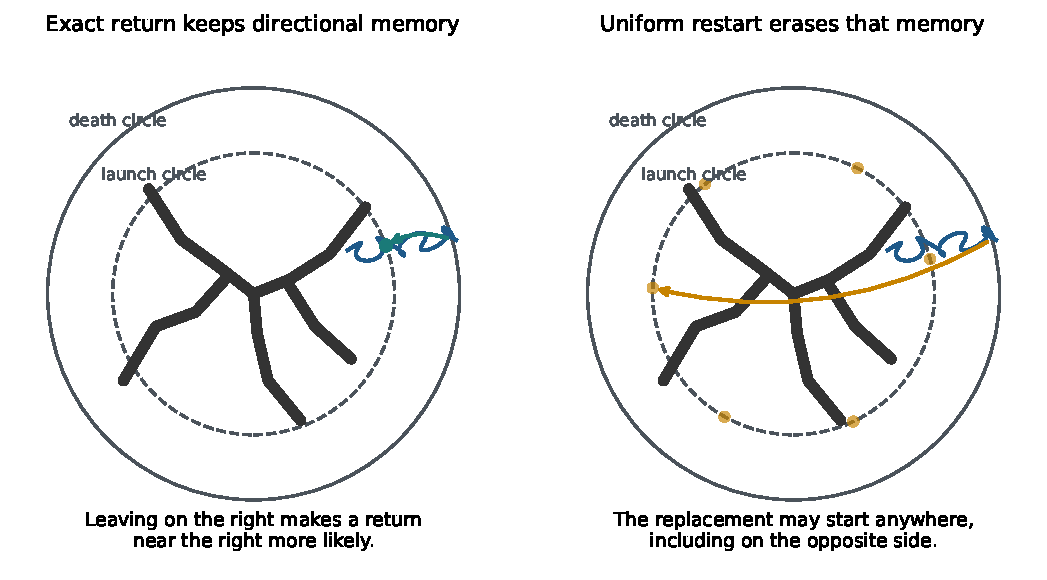
\includegraphics[width=\textwidth]{restart_schematic.pdf}
  \caption{The finite-boundary issue. A Brownian walker that exits on one side is more likely to return on that side. Exact return preserves this directional memory. Uniform restart replaces the returning walker by an angle drawn uniformly around the launch circle.}
  \label{fig:restart}
\end{figure}

A local return distribution can be very nonuniform even when the final attachment bias is small. The aggregate attenuates angular information on the outward journey, and the return kernel attenuates it again on the inward journey. The aim here is to turn that observation into a rigorous statement that remains valid for the nonsmooth compact targets arising in off-lattice DLA.

\subsection{Why the local and global results belong in one paper}

There are two linked questions:

\begin{enumerate}
  \item How far is the approximate next-attachment law from true harmonic measure for a fixed aggregate?
  \item How do those one-step errors affect the law of a complete growing DLA history?
\end{enumerate}

The second question depends directly on the exact identity and norm bounds answering the first. Treating them separately would duplicate the model, notation, prior-art discussion, and central excursion calculation. More importantly, a reader of the global theorem must be able to verify the compact-set identity on which it rests. We therefore present a single self-contained argument, with the smooth-boundary asymptotic refinement placed later because it is informative but not needed for actual disk-union DLA targets.

\subsection{Contributions}

Let $K\subset\C$ be the compact capture target, let
\[
 R_K(c)=\max_{z\in K}|z-c|,
 \qquad
 \rho=\frac{d}{R_K(c)}>1,
\]
and let $\nu_{d,c}$ be the attachment law generated by uniform restart inside the death disk $D(c,d)$. Let $\omega_K$ be harmonic measure from infinity.

The paper establishes the following.

\begin{enumerate}
  \item \textbf{Exact compact-set identity.} For every nonpolar compact target, the bias $\nu_{d,c}-\omega_K$ has an absolutely convergent moment-response expansion in even powers $d^{-2n}$.
  \item \textbf{Birth-radius independence.} The normalized uniform-restart law is independent of the arbitrary launch radius and equals the disk Green equilibrium measure.
  \item \textbf{Self-consistent centering.} For every $K$ and $\rho>1$, there exists $c_\rho\in\conv(K)$ satisfying
  \[
    c_\rho=\int_K z\,\nu_{\rho,c_\rho}(\dd z).
  \]
  \item \textbf{Fourth-order one-step control.} At any such center,
  \[
    \dTV(\nu_{\rho,c_\rho},\omega_K)
    \le \frac{1}{\rho^2(\rho^2-1)}.
  \]
  The exponent four is optimal in general for centering alone, although the universal constants are not claimed to be sharp.
  \item \textbf{A posteriori certification.} The error is bounded by the measured barycenter residual plus the fourth-order remainder; a Hoeffding certificate follows from approximate-law probes alone.
  \item \textbf{Path-space accuracy.} Sequential maximal coupling yields finite- and infinite-horizon total-variation bounds for full DLA growth. For target-radius scaling, a sufficient ideal infinite-horizon schedule is $\rho_n=L n^\alpha$ with $\alpha>1/4$; the amortized theorem later uses the distinct diameter-scaled ratio $\varrho_n$.
  \item \textbf{Honest cost accounting.} The naive distribution-free calibration requires order $\rho^4$ probes to keep sampling uncertainty at fourth-order scale. Near the ideal one-quarter schedule, per-step recalibration is roughly quadratic in the particle horizon.
  \item \textbf{One-shot recentering.} With a diameter-scaled death boundary, one empirical approximate-law barycenter update from any pilot center already gives fourth-order one-step accuracy; no iterative fixed-point solver is required.
  \item \textbf{Amortized center tracking.} For bounded disk growth, the harmonic-measure barycenter has deterministic normalized drift $O(n^{-1/4})$. After an exact finite prefix, or a separately budgeted approximate prefix, blockwise calibration yields a complete infinite-history guarantee with $o(N)$ additional probes through size $N$ whenever $\alpha>11/24$.
\end{enumerate}

\subsection{Novelty boundary}

Harmonic measure, Green equilibrium measures, disk Poisson kernels, moment expansions, conformal centers, maximal coupling, and measurable selection are established tools \cite{Ransford1995,SaffTotik1997,GarnettMarshall2005,Lindvall1992,Kallenberg2021}. Exact circular return and moving centers have also appeared in DLA simulation \cite{MenshutinShchur2006,LeeLuo1992}. The apparently new contribution is the specific combination of:

\begin{itemize}
  \item a finite-law fixed-point center that cancels its own dipole exactly;
  \item an order-sharp geometry-uniform fourth-order total-variation certificate;
  \item a path-space error budget for full DLA growth based on that local theorem;
  \item a one-shot empirical recentering rule that avoids iterative fixed-point solution; and
  \item a deterministic conformal-center drift estimate coupled to a blockwise calibration theorem with sublinear additional probe count.
\end{itemize}

We are not aware of an identical result after a targeted cross-disciplinary search completed in July 2026. Priority remains provisional pending specialist review and exhaustive database searching. The nested-center inequality and deterministic drift estimate are also standalone statements about conformal centers of growing continua, independent of the restart algorithm; they are signposted separately in \cref{sec:center-drift}.

\section{Model and notation}

\subsection{The capture target}

Let $K\subset\C$ be compact, nonpolar, and contain at least two points. Nonpolar means that $K$ has positive logarithmic capacity, which ensures that Brownian hitting and equilibrium measures are nondegenerate. A finite off-lattice DLA capture target, represented by a finite union of closed disks around existing particle centers, satisfies these assumptions even though its boundary can have tangencies and cusps. We write $n_0$ for the number of particles in the prescribed initial seed; all growth histories below are indexed from that seed size.

For a chosen center $c\in\C$, set
\[
  R=R_K(c)=\max_{z\in K}|z-c|.
\]
Choose a death radius $d>R$ and any launch radius $b$ satisfying $R<b<d$.

Let $B_t$ be planar Brownian motion. Write $\tau_K$ for the first hitting time of $K$ and $\tau_d$ for the first hitting time of $\partial D(c,d)$.

\subsection{Exact and approximate attachment laws}

The exact DLA attachment law is harmonic measure from infinity, denoted $\omega_K$. For $f\in C(K)$, if
\[
  h_f(z)=\E_z[f(B_{\tau_K})],
\]
then $h_f$ is bounded and harmonic in the unbounded component of $\C\setminus K$, and
\[
  \omega_K(f)=\lim_{|z|\to\infty}h_f(z).
\]

For one truncated attempt started uniformly on $\partial D(c,b)$, define the subprobability measure
\[
  \mathfrak a_{b,d,c}(A)
  =\Pp(B_{\tau_K}\in A,\ \tau_K<\tau_d),
  \qquad A\subset K.
\]
Let $p_{b,d,c}=\mathfrak a_{b,d,c}(K)$. Because $K$ is nonpolar, its condenser equilibrium potential is strictly positive in $D(c,d)\setminus K$; hence $p_{b,d,c}>0$ for every $R<b<d$. Under uniform restart, failed attempts are discarded and repeated independently until an attachment occurs. Therefore the eventual attachment law is
\begin{equation}
  \nu_{b,d,c}=\frac{\mathfrak a_{b,d,c}}{p_{b,d,c}}.
  \label{eq:restart-conditioned}
\end{equation}
We shall prove that the normalized law does not depend on $b$ and will then write it as $\nu_{d,c}$.

\subsection{Notation guide}

The paper uses two boundary ratios because the static and tracking arguments scale the death circle differently. The symbols are kept distinct throughout.

\begin{center}
\begin{tabularx}{0.96\textwidth}{@{}>{$}l<{$}X@{}}
\toprule
\text{Symbol} & \text{Meaning}\\
\midrule
R_K(c) & \text{smallest radius of a circle centered at $c$ that contains $K$}\\
D(K) & \text{diameter of $K$}\\
\rho=d/R_K(c) & \text{target-radius-scaled death ratio in the fixed-target theory}\\
\varrho=d/D(K) & \text{diameter-scaled death ratio in the amortized tracking theory}\\
\alpha & \text{growth exponent in $\varrho_n=L n^\alpha$}\\
\gamma & \text{normalized calibration-accuracy exponent}\\
\chi,\delta_k,\delta_{\mathrm{cal}} & \text{one-shot failure level, block allocations, and total calibration-failure budget}\\
n_0,\tau_0 & \text{seed size and first blockwise-calibration size}\\
\mathfrak a_{b,d,c} & \text{one-attempt attachment submeasure before the death circle is reached}\\
\omega_K,\nu_{d,c} & \text{exact harmonic measure and finite-boundary uniform-restart law}\\
\bottomrule
\end{tabularx}
\end{center}

\subsection{Total variation and complex moments}

For probability measures $\mu$ and $\lambda$ on the same measurable space,
\[
  \dTV(\mu,\lambda)
  =\sup_A|\mu(A)-\lambda(A)|
  =\frac12\norm{\mu-\lambda}_{\mathrm{var}}.
\]
This is the strongest common probability metric used here: it controls the difference in probability assigned to every event and every bounded statistic.

For a probability measure $\mu$ on $K$, define its complex moments about $c$ by
\begin{equation}
  M_n^c(\mu)=\int_K(z-c)^n\,\mu(\dd z),
  \qquad n\ge1.
  \label{eq:moments}
\end{equation}
The first moment is the displacement of the measure's barycenter from $c$.

\begin{plainbox}
The first moment is the broadest possible directional imbalance: more attachment probability on one side than the other. In electrostatic language it is a dipole. Higher moments describe twofold, threefold, and finer angular structure.
\end{plainbox}

\section{Uniform restart and Green equilibrium}

\begin{proposition}[Independence of the launch radius]
\label{prop:birth-independent}
For fixed $K$, $c$, and $d$, the normalized law in \eqref{eq:restart-conditioned} is independent of every launch radius $b\in(R,d)$.
\end{proposition}

\begin{proof}
For $f\in C(K)$, define the killed harmonic extension
\[
  u_f(z)=\E_z[f(B_{\tau_K});\ \tau_K<\tau_d]
\]
in $D(c,d)\setminus K$. On each circle $|z-c|=r$ with $R<r<d$, let
\[
  A_f(r)=\frac{1}{2\pi}\int_0^{2\pi}
  u_f(c+re^{i\theta})\dd\theta.
\]
Because the full circle lies in the harmonic region, differentiating under the integral and using the polar Laplacian gives
\[
  A_f''(r)+\frac1rA_f'(r)=0.
\]
Since $u_f=0$ on the death circle, $A_f(d)=0$, so
\[
  A_f(r)=a_f\log(d/r)
\]
for a constant $a_f$. The same calculation with $f\equiv1$ gives $A_1(r)=a_1\log(d/r)$. Therefore
\[
  \nu_{b,d,c}(f)=\frac{A_f(b)}{A_1(b)}=\frac{a_f}{a_1},
\]
which is independent of $b$.
\end{proof}

\begin{remark}[Uniform relaunch on the death circle]
Some legacy implementations describe their reset as occurring on the death circle rather than on a distinct inner launch circle. Any such code has an effective relaunch radius $b<d$ once its finite numerical step or inward offset is made explicit. By launch-radius independence, every effective $b\in(R,d)$ produces the same normalized attachment law and the same certificate. The formal limit $b\uparrow d$ therefore covers these implementations without treating continuum Brownian motion as starting on an absorbing boundary.
\end{remark}

\begin{proposition}[Green-equilibrium identification]
\label{prop:green-equilibrium}
The common law $\nu_{d,c}$ is the Green equilibrium measure of $K$ relative to the disk $D(c,d)$.
\end{proposition}

\begin{proof}
Let $\sigma_b$ be uniform probability measure on the launch circle $\partial D(c,b)$, and let $g_{d,c}$ be the Green function of $D(c,d)$. Its Green potential is
\[
  U_{d,c}^{\sigma_b}(w)
  =\int g_{d,c}(z,w)\,\sigma_b(\dd z).
\]
For $|w-c|<b$, Jensen's circular-mean formula applied to the two logarithmic terms in $g_{d,c}$ gives
\[
  \frac1{2\pi}\int_0^{2\pi}
  \log\left|d^2-be^{i\theta}\overline{(w-c)}\right|\dd\theta
  =2\log d,
\]
and
\[
  \frac1{2\pi}\int_0^{2\pi}
  \log|c+be^{i\theta}-w|\dd\theta
  =\log b.
\]
Hence
\begin{equation}
  U_{d,c}^{\sigma_b}(w)=\log(d/b),
  \qquad |w-c|<b.
  \label{eq:launch-potential-constant}
\end{equation}

Let $\tau=\tau_K\wedge\tau_d$. For quasi-every $w\in K$, the function $z\mapsto g_{d,c}(z,w)$ is nonnegative and harmonic on $D(c,d)\setminus K$. To justify equality rather than only a supermartingale inequality, first stop on an increasing exhaustion of $D(c,d)\setminus\bigl(K\cup\overline{D(w,1/m)}\bigr)$, where $z\mapsto g_{d,c}(z,w)$ is bounded and harmonic and its death-circle boundary value is zero. Optional stopping on the exhausted domains, followed by monotone convergence as the exhaustion fills the domain and $m\to\infty$, gives
\[
  g_{d,c}(z,w)
  =\E_z\!\left[g_{d,c}(B_{\tau_K},w);\ \tau_K<\tau_d\right].
\]
Irregular boundary points of $K$ form a polar exceptional set and are not charged by Brownian hitting measure, so the quasi-everywhere boundary values suffice.
Average this identity over $z\sim\sigma_b$ and use Tonelli's theorem. By the definition of the one-attempt hitting submeasure,
\begin{equation}
  U_{d,c}^{\mathfrak a_{b,d,c}}(w)
  =U_{d,c}^{\sigma_b}(w)
  =\log(d/b)
  \quad\text{for quasi-every }w\in K.
  \label{eq:balayage-potential}
\end{equation}
This is precisely the Green-balayage identity, obtained here directly from Brownian stopping. Brownian hitting measures do not charge polar sets, so after division by
$p_{b,d,c}=\mathfrak a_{b,d,c}(K)>0$, the probability measure
$\nu_{b,d,c}$ has finite Green energy and constant Green potential quasi-everywhere on $K$.

For completeness, this constant-potential property characterizes the equilibrium measure. If $\mu\in\mathcal P(K)$ has finite Green energy and $C$ is the quasi-everywhere constant potential of $\nu_{b,d,c}$, then
\[
  I_{d,c}(\mu,\nu_{b,d,c})=C=I_{d,c}(\nu_{b,d,c}).
\]
Positive definiteness of Green energy therefore gives
\[
  I_{d,c}(\mu)-I_{d,c}(\nu_{b,d,c})
  =I_{d,c}(\mu-\nu_{b,d,c})\ge0.
\]
Competitors of infinite energy are irrelevant. Thus $\nu_{b,d,c}$ is the unique Green-energy minimizer, hence the Green equilibrium measure. This also provides a second proof of launch-radius independence. Background on balayage, polar exceptional sets, and the Frostman characterization may be found in \cite[Chs.~4--5]{Ransford1995} and \cite[Part~I]{SaffTotik1997}.
\end{proof}

\begin{plainbox}
Uniform restart does not produce a mysterious new probability law. It produces the equilibrium measure appropriate to a finite grounded outer disk. Exact DLA uses the corresponding equilibrium measure when the outer boundary is infinitely far away. The problem is therefore a finite-domain versus infinite-domain comparison.
\end{plainbox}

\section{An exact excursion identity for arbitrary compact targets}

\subsection{Exterior response measures}

For $f\in C(K)$, the full harmonic extension $h_f(z)=\E_z[f(B_{\tau_K})]$ is harmonic outside the disk $|z-c|\le R$ and bounded at infinity. It therefore has the convergent expansion
\begin{equation}
  h_f(c+re^{i\theta})
  =\omega_K(f)
  +2\Real\sum_{n=1}^{\infty}
     \eta_n^c(f)\,r^{-n}e^{-in\theta},
  \qquad r>R.
  \label{eq:exterior-expansion}
\end{equation}
For each $n$, $f\mapsto\eta_n^c(f)$ is a bounded complex linear functional on $C(K)$ and hence a complex measure. Moreover,
\begin{equation}
  \norm{\eta_n^c}_{\mathrm{var}}\le R^n.
  \label{eq:eta-bound}
\end{equation}
Indeed, the $n$th Fourier coefficient on a circle of radius $r$ is $r^{-n}\eta_n^c(f)$ and has magnitude at most $\norm{f}_\infty$; let $r\downarrow R$.

\subsection{The exact identity}

\begin{theorem}[Exact finite-boundary bias identity]
\label{thm:exact-identity}
For every compact nonpolar $K$, center $c$, and death radius $d>R_K(c)$, the uniform-restart and exact attachment laws satisfy, for every real $f\in C(K)$,
\begin{equation}
\boxed{
  \int_K f\,\dd(\nu_{d,c}-\omega_K)
  =2\Real\sum_{n=1}^{\infty}
     d^{-2n}\,
     \overline{M_n^c(\nu_{d,c})}\,
     \eta_n^c(f).
}
\label{eq:exact-weak}
\end{equation}
The series converges absolutely and uniformly over $\norm{f}_\infty\le1$.
\end{theorem}

\begin{proof}
Choose any $b\in(R,d)$ and write $q=b/d$. For a launch angle $\theta$, let $H_\theta$ be the full, unrestricted attachment law on $K$ of Brownian motion started at $c+be^{i\theta}$. For $f\in C(K)$ define
\[
  H_n(f)=\frac1{2\pi}\int_0^{2\pi}e^{in\theta}H_\theta(f)\dd\theta,
  \qquad n\in\mathbb Z.
\]
The constant angular mode is the exact law:
\begin{equation}
  H_0(f)=\frac1{2\pi}\int_0^{2\pi}H_\theta(f)\dd\theta
  =\omega_K(f).
  \label{eq:circle-average-exact}
\end{equation}
Indeed, the circular mean of the bounded exterior harmonic function $h_f$ is independent of radius and equals its value at infinity; equivalently, Brownian motion arriving from infinity first hits every centered enclosing circle with uniform angle. By \eqref{eq:exterior-expansion},
\begin{equation}
  b^nH_n=\eta_n^c,
  \qquad n\ge1.
  \label{eq:Hn-eta}
\end{equation}

For one truncated attempt, write $\mathfrak a=\mathfrak a_{b,d,c}$, $p=\mathfrak a(K)$, and let $\epsilon$ be the subprobability law of the death-circle exit angle $\phi$ on the event $\tau_d<\tau_K$. Thus $\epsilon([0,2\pi))=1-p$. Optional stopping of the bounded complex martingale $(B_t-c)^n$ at $\tau_K\wedge\tau_d$ gives
\begin{equation}
  \int e^{in\phi}\epsilon(\dd\phi)
  =-d^{-n}M_n^c(\mathfrak a),
  \qquad n\ge1.
  \label{eq:outward-mode}
\end{equation}
The initial expectation vanishes because the launch angle is uniform.

A path that reaches $\partial D(c,d)$ returns to the inner circle $\partial D(c,b)$ almost surely by recurrence of planar Brownian motion. Conditional on death-circle angle $\phi$, its return angle $\theta$ has density, relative to uniform angular measure,
\begin{equation}
  P_q(\theta-\phi)
  =1+\sum_{n=1}^{\infty}q^n
  \left(e^{in(\theta-\phi)}+e^{-in(\theta-\phi)}\right).
  \label{eq:poisson-series}
\end{equation}
The series converges absolutely and uniformly because $q<1$.

Apply the strong Markov property at the first hit of $K$ or the death circle. Starting uniformly on the launch circle and then allowing exact continuation gives the unrestricted law $\omega_K$, so for every real $f\in C(K)$,
\begin{align}
  \omega_K(f)
  ={}&\mathfrak a(f)
  +\int\epsilon(\dd\phi)
    \frac1{2\pi}\int_0^{2\pi}
      P_q(\theta-\phi)H_\theta(f)\dd\theta.
  \label{eq:renewal-before-fourier}
\end{align}
The constant Fourier mode in \eqref{eq:poisson-series}, together with \eqref{eq:circle-average-exact}, contributes exactly $(1-p)\omega_K(f)$. The remaining modes give
\begin{align}
  p\omega_K(f)
  ={}&\mathfrak a(f)
  +\sum_{n\ge1}q^n
  \left[
    \left(\int e^{-in\phi}\epsilon(\dd\phi)\right)H_n(f)
    +\left(\int e^{in\phi}\epsilon(\dd\phi)\right)H_{-n}(f)
  \right].
  \label{eq:renewal-fourier}
\end{align}
Substituting \eqref{eq:outward-mode}, using $\mathfrak a=p\nu_{d,c}$, and then using \eqref{eq:Hn-eta}, yields
\[
  \nu_{d,c}(f)-\omega_K(f)
  =2\Real\sum_{n=1}^{\infty}
    d^{-2n}\overline{M_n^c(\nu_{d,c})}\eta_n^c(f),
\]
which is \eqref{eq:exact-weak}.

The exchanges of the Fourier sum with the angular and exit expectations are justified by the uniform absolute convergence of \eqref{eq:poisson-series}. The final series is uniformly absolutely convergent for $\norm{f}_\infty\le1$ because
\[
  |M_n^c(\nu_{d,c})|\le R^n,
  \qquad
  \norm{\eta_n^c}_{\mathrm{var}}\le R^n,
  \qquad
  \sum_{n\ge1}(R/d)^{2n}<\infty.
\]
\end{proof}

\subsection{A compact-target Neumann expansion}

The exact identity is implicit because the moments on its right-hand side are moments of the approximate law itself. It can nevertheless be inverted directly when the death circle is sufficiently distant.

For a finite real signed measure $\mu$ on $K$, define the real signed measure
\begin{equation}
  \mathcal L_n^c\mu
  =\overline{M_n^c(\mu)}\,\eta_n^c
   +M_n^c(\mu)\,\overline{\eta_n^c},
  \qquad n\ge1,
  \label{eq:Ln-operator}
\end{equation}
The conjugation convention in \eqref{eq:Ln-operator} is the same as in \eqref{eq:exact-weak}: the coefficient multiplying $\eta_n^c$ is $\overline{M_n^c(\mu)}$. This convention is used throughout the Neumann expansion and the sharpness calculation.
Set
\begin{equation}
  T_{d,c}=\sum_{n\ge1}d^{-2n}\mathcal L_n^c.
  \label{eq:T-operator}
\end{equation}
Then \cref{thm:exact-identity} is the measure equation
\begin{equation}
  \nu_{d,c}-\omega_K=T_{d,c}\nu_{d,c}.
  \label{eq:operator-equation}
\end{equation}

\begin{theorem}[Compact-target multipole expansion]
\label{thm:compact-neumann}
Let $s=(R_K(c)/d)^2$. If $s<1/3$, then $I-T_{d,c}$ is invertible on finite signed measures in variation norm and
\begin{equation}
  \nu_{d,c}=(I-T_{d,c})^{-1}\omega_K.
  \label{eq:neumann-solution}
\end{equation}
Suppose, for some $m\ge1$,
\[
  M_1^c(\omega_K)=\cdots=M_{m-1}^c(\omega_K)=0.
\]
Then, as $d\to\infty$ with $K$ and $c$ fixed,
\begin{equation}
  \nu_{d,c}-\omega_K
  =d^{-2m}\mathcal L_m^c\omega_K
   +O_{\mathrm{var}}(d^{-2m-2}).
  \label{eq:compact-leading}
\end{equation}
If $\mathcal L_m^c\omega_K\ne0$, then
\begin{equation}
  \dTV(\nu_{d,c},\omega_K)
  =C_m d^{-2m}+O(d^{-2m-2}),
  \qquad
  C_m=\tfrac12\norm{\mathcal L_m^c\omega_K}_{\mathrm{var}}>0.
  \label{eq:compact-two-sided}
\end{equation}
\end{theorem}

\begin{proof}
For every signed measure $\mu$,
\[
  |M_n^c(\mu)|\le R^n\norm{\mu}_{\mathrm{var}},
  \qquad
  \norm{\eta_n^c}_{\mathrm{var}}\le R^n,
\]
so
\[
  \norm{\mathcal L_n^c\mu}_{\mathrm{var}}
  \le2R^{2n}\norm{\mu}_{\mathrm{var}}.
\]
Consequently
\[
  \norm{T_{d,c}}
  \le2\sum_{n\ge1}s^n
  =\frac{2s}{1-s}<1
\]
when $s<1/3$. The Neumann series proves \eqref{eq:neumann-solution}. Under the moment assumptions, $\mathcal L_n^c\omega_K=0$ for $n<m$, hence
\[
  T_{d,c}\omega_K
  =d^{-2m}\mathcal L_m^c\omega_K
   +O_{\mathrm{var}}(d^{-2m-2}).
\]
Since $(I-T_{d,c})^{-1}=I+O(d^{-2})$ in operator norm, \eqref{eq:compact-leading} follows. Taking variation norms gives \eqref{eq:compact-two-sided} when the displayed leading measure is nonzero.
\end{proof}

\begin{remark}[What is and is not proved for arbitrary compacta]
\label{rem:compact-tradeoff}
For general compact targets, \cref{thm:compact-neumann} gives an upper-order statement unless the response measure $\mathcal L_m^c\omega_K$ is known to be nonzero. A nonzero equilibrium moment $M_m^c(\omega_K)$ does not, by itself, make that implication automatic at this level of generality. For $C^{2,\sigma}$ Jordan boundaries, however, \cref{thm:smooth-asymptotic} proves that the leading coefficient is nonzero whenever the first nonvanishing equilibrium moment is of order $m$. Thus the compact theory supplies the DLA-relevant bounds, while the smooth theory supplies the full two-sided generic asymptotic.
\end{remark}

\begin{plainbox}
The exponent is doubled because the same angular signal is weakened twice: once while traveling from the target to the death circle, and once while returning. An order-$n$ pattern contributes at scale $(R/d)^n(R/d)^n=(R/d)^{2n}$.
\end{plainbox}

\subsection{Immediate one-step bounds}

Put
\[
  s=\left(\frac{R}{d}\right)^2.
\]

\begin{proposition}[Generic and residual bounds]
\label{prop:residual-bounds}
For every center $c$ and $d>R$,
\begin{equation}
  \dTV(\nu_{d,c},\omega_K)
  \le \min\left\{1,\frac{s}{1-s}\right\}.
  \label{eq:generic-bound}
\end{equation}
If
\[
  e_d(c)=\left|\int_K(z-c)\,\nu_{d,c}(\dd z)\right|,
\]
then the sharper residual bound is
\begin{equation}
\boxed{
  \dTV(\nu_{d,c},\omega_K)
  \le \min\left\{1,
  \frac{e_d(c)R}{d^2}+\frac{s^2}{1-s}
  \right\}.
}
\label{eq:residual-bound}
\end{equation}
\end{proposition}

\begin{proof}
Apply \eqref{eq:exact-weak} with $\norm{f}_\infty\le1$. The full series is bounded in signed-measure variation by $2\sum_{n\ge1}s^n$; dividing by two gives \eqref{eq:generic-bound}. For \eqref{eq:residual-bound}, bound the $n=1$ contribution by $e_d(c)R/d^2$ in probability total variation and sum the tail $\sum_{n\ge2}s^n=s^2/(1-s)$. Total variation never exceeds one.
\end{proof}

\section{The self-consistent restart center}

\subsection{Definition and intuition}

Fix a radius ratio $\rho>1$. For $c\in\conv(K)$, set
\[
  d_\rho(c)=\rho R_K(c)
\]
and let $\nu_{\rho,c}=\nu_{d_\rho(c),c}$. Define the finite-law barycenter map
\begin{equation}
  \Phi_\rho(c)=\int_K z\,\nu_{\rho,c}(\dd z).
  \label{eq:phi-map}
\end{equation}

\begin{definition}[Self-consistent restart center]
A point $c_\rho\in\conv(K)$ is self-consistent if
\begin{equation}
  \Phi_\rho(c_\rho)=c_\rho.
  \label{eq:self-consistency}
\end{equation}
\end{definition}

\begin{figure}[H]
  \centering
  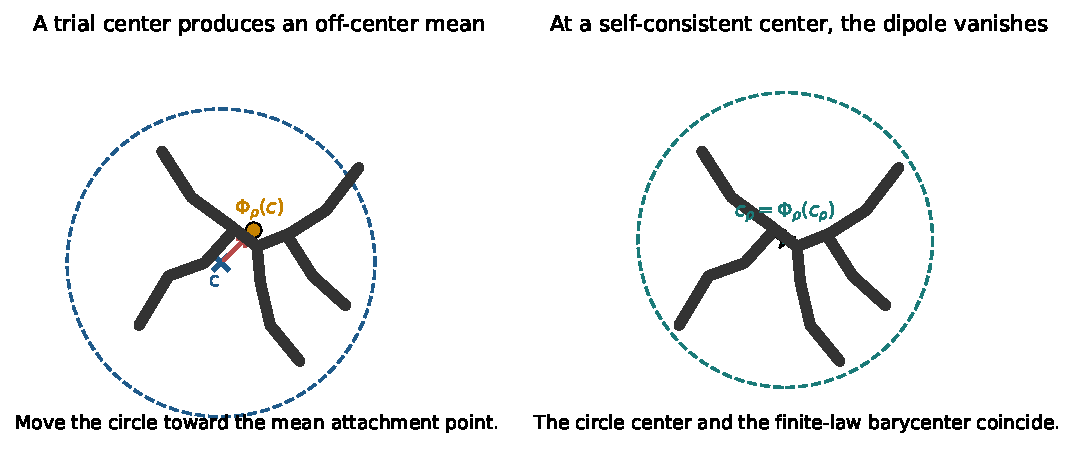
\includegraphics[width=\textwidth]{self_center_schematic.pdf}
  \caption{The self-consistency condition. A trial center can produce a finite-boundary attachment law whose mean lies elsewhere. A self-consistent center is a fixed point of this barycenter map. At that point the first complex moment of the approximate law is exactly zero.}
  \label{fig:self-center}
\end{figure}

Unlike the harmonic-measure barycenter, which is defined using the exact law, $c_\rho$ is defined entirely through the approximate law that the simulator can sample.

\subsection{Existence}

\begin{theorem}[Existence of a self-consistent center]
\label{thm:self-center-existence}
For every compact nonpolar $K\subset\C$ containing at least two points and every $\rho>1$, the map $\Phi_\rho$ has at least one fixed point in $\conv(K)$.
\end{theorem}

\begin{proof}
Let $C=\conv(K)$. Because $\nu_{\rho,c}$ is a probability measure supported on $K$, its barycenter lies in $C$, so $\Phi_\rho:C\to C$.

We prove continuity. Let $c_j\to c$ in $C$, write $d_j=\rho R_K(c_j)$ and $d=\rho R_K(c)$. The disk Green kernel is
\[
  g_j(z,w)=
  \log\left|
  \frac{d_j^2-(z-c_j)\overline{(w-c_j)}}
       {d_j(z-w)}
  \right|.
\]
Separate the singular part $-\log|z-w|$, which is independent of $j$, from the regular part. Since
\[
  |(z-c_j)\overline{(w-c_j)}|
  \le R_K(c_j)^2=\rho^{-2}d_j^2,
\]
the logarithm in the regular part remains uniformly away from zero by the fixed factor $1-\rho^{-2}$. The function $c\mapsto R_K(c)$ is continuous, and it is bounded below on $C$ by half the diameter of $K$. Hence the regular parts converge uniformly on $K\times K$.

Let $I_j$ and $I$ be the corresponding Green-energy functionals on the weakly compact space $\mathcal P(K)$ of probability measures on $K$. Let $\nu_j$ minimize $I_j$. Any subsequence has a weakly convergent subsubsequence, say $\nu_{j_k}\Rightarrow\nu$. Lower semicontinuity of logarithmic energy and uniform convergence of the regular parts give
\[
  I(\nu)\le\liminf_{k\to\infty}I_{j_k}(\nu_{j_k}).
\]
For every competitor $\mu\in\mathcal P(K)$ of finite energy,
\[
  I_{j_k}(\nu_{j_k})\le I_{j_k}(\mu)\longrightarrow I(\mu).
\]
Thus $I(\nu)\le I(\mu)$ for every competitor, so $\nu$ is the Green equilibrium measure for $c$. That minimizer is unique. Therefore every convergent subsubsequence has the same limit and
\[
  \nu_{\rho,c_j}\Rightarrow\nu_{\rho,c}.
\]
The barycenter is continuous under weak convergence on compact $K$, hence $\Phi_\rho(c_j)\to\Phi_\rho(c)$.

The set $C$ is compact and convex. Brouwer's fixed-point theorem now gives a point $c_\rho$ satisfying \eqref{eq:self-consistency}.
\end{proof}

\begin{remark}
The point $c_\rho$ may lie inside $K$. This causes no difficulty: it is the center of the enclosing computational circles, not a starting point for the Brownian walker. Any launch circle with radius greater than $R_K(c_\rho)$ lies outside the entire target.
\end{remark}

\begin{remark}
Existence does not imply uniqueness, contraction of $\Phi_\rho$, or fast convergence of an iteration $c\leftarrow\Phi_\rho(c)$. Those are separate algorithmic questions.
\end{remark}

\begin{technicalbox}[title={Conceptual and algorithmic roles}]
The exact fixed point explains why fourth-order cancellation is possible and supplies an ideal comparison kernel. It is not required by the implementable tracking scheme: \cref{prop:one-shot} shows that one empirical approximate-law barycenter update already restores fourth-order one-step accuracy. The measurable-selection machinery later in the paper is therefore used only to formalize the ideal self-centered process, not as a proposed numerical solver.
\end{technicalbox}

\subsection{Fourth-order cancellation}

\begin{theorem}[Residual certificate and exact cancellation]
\label{thm:self-centered-bound}
For any trial center $c\in\conv(K)$, with $R=R_K(c)$ and $d=\rho R$,
\begin{equation}
\boxed{
  \dTV(\nu_{\rho,c},\omega_K)
  \le
  \min\left\{1,
  \rho^{-2}\frac{|\Phi_\rho(c)-c|}{R}
  +\frac{1}{\rho^2(\rho^2-1)}
  \right\}.
}
\label{eq:ratio-residual}
\end{equation}
At every self-consistent center $c_\rho$,
\begin{equation}
\boxed{
  \dTV(\nu_{\rho,c_\rho},\omega_K)
  \le
  \eps_\star(\rho)
  :=\min\left\{1,
  \frac{1}{\rho^2(\rho^2-1)}
  \right\}.
}
\label{eq:self-centered-epsilon}
\end{equation}
In particular,
\[
  \eps_\star(\rho)=\rho^{-4}+O(\rho^{-6})
  \qquad(\rho\to\infty).
\]
\end{theorem}

\begin{proof}
The residual is precisely the first moment:
\[
  M_1^c(\nu_{\rho,c})=\Phi_\rho(c)-c.
\]
Substitute $d=\rho R$ into \eqref{eq:residual-bound}. At a fixed point the residual vanishes exactly.
\end{proof}

\begin{figure}[H]
  \centering
  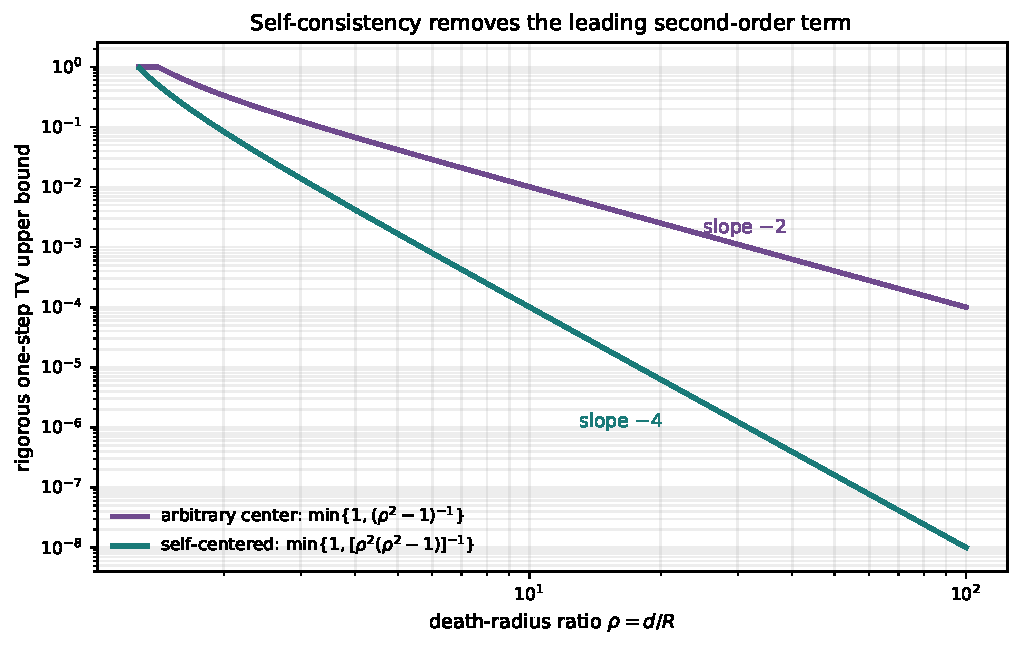
\includegraphics[width=0.87\textwidth]{local_bounds.pdf}
  \caption{Rigorous one-step upper bounds. At an arbitrary center the generic guarantee is second order. A self-consistent center removes the dipole and leaves a fourth-order remainder. The bounds are worst-case and can be much larger than observed errors.}
  \label{fig:local-bounds}
\end{figure}

\begin{plainbox}
If the death circle is moved twice as far away relative to the cluster, a second-order error becomes about four times smaller. A fourth-order error becomes about sixteen times smaller. The self-consistency condition changes the guaranteed power, not merely a numerical prefactor.
\end{plainbox}

\subsection{Relation to the true growth-probability center}

Define the harmonic-measure barycenter
\[
  c_H=\int_K z\,\omega_K(\dd z).
\]
For a simply connected exterior, $c_H$ is the constant Laurent coefficient of the normalized exterior conformal map \cite{DavidovitchEtAl1999}. It is a classical geometric quantity; the contribution here is the finite-law fixed point and its error-cancellation role.

\begin{corollary}[Self-centers approach the harmonic center]
\label{cor:center-closeness}
At any self-consistent center $c_\rho$, with $R=R_K(c_\rho)$,
\[
  |c_\rho-c_H|
  \le 2R\,\eps_\star(\rho).
\]
\end{corollary}

\begin{proof}
Because both measures have mass one,
\[
  c_\rho-c_H
  =\int_K(z-c_\rho)\,\dd(\nu_{\rho,c_\rho}-\omega_K).
\]
The integrand has magnitude at most $R$, so the result follows from
$\norm{\nu-\omega}_{\mathrm{var}}=2\dTV(\nu,\omega)$ and \eqref{eq:self-centered-epsilon}.
\end{proof}

\subsection{The fourth-order exponent is sharp}

\begin{proposition}[A target with a nonzero fourth-order term]
\label{prop:sharpness}
Let $K=[-a,a]$ and use the symmetric center $c=0$, which is self-consistent for every $d>a$. Then, as $d\to\infty$,
\[
  \int_K\frac{x^2}{a^2}\,
  (\nu_{d,0}-\omega_K)(\dd x)
  =\frac{a^4}{16d^4}+O(d^{-6}).
\]
Consequently,
\[
  \dTV(\nu_{d,0},\omega_K)
  \ge\frac{a^4}{32d^4}+O(d^{-6}).
\]
Thus no universal centering rule can improve circular uniform restart beyond fourth order without also correcting higher angular modes.
\end{proposition}

\begin{proof}
Harmonic measure from infinity on $[-a,a]$ is the arcsine law, so
\[
  M_2^0(\omega_K)=\frac{a^2}{2}.
\]
For $f(x)=x^2/a^2$, the Joukowski map
\[
  w=\frac{z+\sqrt{z^2-a^2}}{a}
\]
maps the exterior of the segment to $|w|>1$. On the segment, $x=a\cos\theta$ and $f=(1+\cos2\theta)/2$, so its exterior harmonic extension is
\[
  h_f(z)=\frac12+\frac12\Real(w^{-2}).
\]
Since $w^{-2}=a^2/(4z^2)+O(z^{-4})$, the normalization in \eqref{eq:exterior-expansion} gives $\eta_2^0(f)=a^2/16$. Symmetry kills odd modes. Substituting the $n=2$ term into \eqref{eq:exact-weak} gives the displayed expansion; replacing $M_2(\nu)$ by $M_2(\omega)$ affects only higher order. The total-variation lower bound follows because $|f|\le1$.
\end{proof}

\section{A data-driven residual certificate}

A simulator need not solve \eqref{eq:self-consistency} exactly. It can estimate the finite-law barycenter using independent uniform-restart probes.

Let $X_1,\ldots,X_M$ be independent attachment points with law $\nu_{\rho,c}$ and define
\[
  \widehat\Phi_M(c)=\frac1M\sum_{j=1}^M X_j.
\]

\begin{corollary}[Monte Carlo certificate]
\label{cor:monte-carlo}
For every confidence level $1-\eta$, with probability at least $1-\eta$,
\begin{equation}
\boxed{
\begin{aligned}
  \dTV(\nu_{\rho,c},\omega_K)
  \le{}&
  \rho^{-2}
  \left[
    \frac{|\widehat\Phi_M(c)-c|}{R}
    +2\sqrt{\frac{\log(4/\eta)}{M}}
  \right]
  \\
  &+\frac{1}{\rho^2(\rho^2-1)},
\end{aligned}
}
\label{eq:mc-certificate}
\end{equation}
with the right-hand side capped at one.
\end{corollary}

\begin{proof}
Each coordinate of $X_j-c$ lies in $[-R,R]$. Hoeffding's inequality and a union bound over the two coordinates imply \cite{Hoeffding1963}
\[
  \Pp\left(
  |\widehat\Phi_M(c)-\Phi_\rho(c)|
  >2R\sqrt{\frac{\log(4/\eta)}{M}}
  \right)\le\eta.
\]
On the complementary event, apply the triangle inequality to the true residual and substitute into \eqref{eq:ratio-residual}.
\end{proof}

\begin{costbox}
The certificate is rigorous but conservative. To make the sampling term no larger than the fourth-order remainder, even when the empirical residual is negligible, it is sufficient---and is the natural worst-case scale for a distribution-free Hoeffding certificate---that
\[
  M\gtrsim4(\rho^2-1)^2\log(4/\eta)
  \sim4\rho^4\log(4/\eta).
\]
No uniform empirical-variance improvement is possible without additional assumptions: probability laws supported near opposite extremal points can have coordinate variance of order $R^2$. Thus the $\rho^4$ scaling is necessary for this distribution-free Hoeffding certificate up to constants and logarithms; it is not claimed to be a lower bound for every estimator. A fresh such calibration at every attachment can be much more expensive than exact Poisson return.
\end{costbox}

\begin{figure}[H]
  \centering
  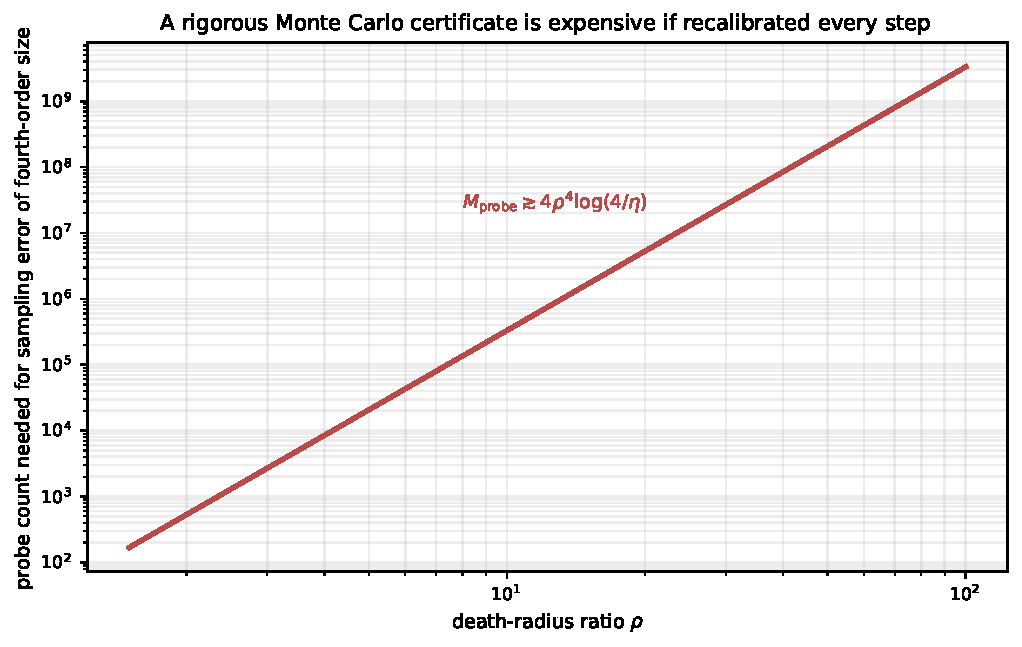
\includegraphics[width=0.82\textwidth]{calibration_cost.pdf}
  \caption{Probe complexity of the distribution-free certificate. The plot shows the count required to make the Hoeffding sampling term comparable to the fourth-order deterministic remainder at confidence $1-10^{-3}$. It is a worst-case calibration cost, not a claim about an optimized stochastic-approximation scheme.}
  \label{fig:calibration-cost}
\end{figure}

The theorem certifies any trial center. It does not prove that $c\leftarrow\widehat\Phi_M(c)$ is a contraction, that the fixed point is unique, or that a particular numerical solver converges quickly. Variance-sensitive bounds, probe reuse, conformal estimates, and infrequent recalibration may be far cheaper, but require separate analysis.

\section{From one attachment to the full DLA history}

\subsection{State spaces and transition kernels}

Let $\mathsf S_n$ be a standard Borel state space of $n$-particle aggregates. In a concrete off-lattice implementation, a state can be represented by an ordered vector of particle centers together with a deterministic convention for resolving multiple contacts. Let $K(A)$ be the capture target for the next particle.

Let
\[
  P_n(A,\cdot)
\]
be the exact DLA transition kernel obtained from $\omega_{K(A)}$, and let
\[
  Q_n(A,\cdot)
\]
be a measurable finite-boundary restart kernel. Pushing attachment measures through the measurable map that adds the next particle cannot increase total variation.

The existence of a self-center is pointwise. To define a Markov kernel one also needs a measurable choice.

\begin{assumption}[Measurable self-center framework]
\label{ass:measurable}
For each $n$, the map $(A,c)\mapsto\Phi_{\rho_n,A}(c)$ is jointly Borel on the graph of $c\in\conv K(A)$ and continuous in $c$; the convex-hull correspondence $A\mapsto\conv K(A)$ has a Borel graph.
\end{assumption}

These conditions hold in the usual finite-coordinate formulation once the Brownian hitting kernel and geometric tie-breaking rules are taken as measurable. They are stated explicitly so the path-law theorem does not hide a selection issue.

\begin{proposition}[Measurable choice of a self-center]
\label{prop:measurable-selector}
Under \cref{ass:measurable}, there is a Borel map $A\mapsto c_n(A)$ such that
\[
  c_n(A)\in\conv K(A),
  \qquad
  \Phi_{\rho_n,A}(c_n(A))=c_n(A).
\]
\end{proposition}

\begin{proof}
The fixed-point correspondence has a Borel graph and nonempty compact sections. The Arsenin--Kunugui uniformization theorem therefore supplies a Borel selector; the verification is given in \cref{app:selector-proof}. This is the precise compact-section uniformization step, rather than an unqualified appeal to measurable selection.
\end{proof}

\subsection{Measurable maximal coupling}

\begin{lemma}[Kernelwise maximal coupling]
\label{lem:maximal-kernel-coupling}
Let $P(x,\cdot)$ and $Q(x,\cdot)$ be probability kernels from a standard Borel space into another standard Borel space. There exists a jointly measurable coupling kernel $\Gamma(x,\dd y,\dd z)$ whose marginals are $P$ and $Q$ and for which
\[
  \Gamma_x\{y=z\}=1-\dTV(P_x,Q_x).
\]
\end{lemma}

\begin{proof}
Let $\lambda_x=P_x+Q_x$. The measurable Radon--Nikodym theorem gives jointly measurable densities $p(x,y)$ and $q(x,y)$ with respect to the kernel $\lambda_x$ \cite{Kallenberg2021}. Define the common subprobability kernel
\[
  C_x(A)=\int_A\min\{p(x,y),q(x,y)\}\,\lambda_x(\dd y)
\]
and put $t(x)=1-C_x(\mathsf Y)$. Then
\[
  t(x)=\dTV(P_x,Q_x),
\]
and the residual kernels $P_x-C_x$ and $Q_x-C_x$ both have mass $t(x)$. Let $\Delta C_x$ denote the diagonal lift of $C_x$, characterized by
\[
  \Delta C_x(A\times B)=C_x(A\cap B).
\]
If $t(x)>0$, set
\[
  \Gamma_x
  =\Delta C_x
   +\frac{(P_x-C_x)\otimes(Q_x-C_x)}{t(x)};
\]
if $t(x)=0$, set $\Gamma_x=\Delta P_x$. Every operation in this formula is measurable in $x$, so $\Gamma$ is a probability kernel. Its marginals are $P_x$ and $Q_x$, while the residual product term gives no additional diagonal mass because its two factors are mutually singular by construction. Hence
\[
  \Gamma_x\{y=z\}=C_x(\mathsf Y)=1-\dTV(P_x,Q_x).
\]
This is the standard maximal-coupling construction \cite{Lindvall1992,Thorisson2000}.
\end{proof}

\subsection{Sequential coupling}

\begin{theorem}[Finite-horizon path-space bound]
\label{thm:path-bound}
Suppose exact and approximate growth processes start from the same seed and, for every $A\in\mathsf S_n$,
\[
  \dTV(P_n(A,\cdot),Q_n(A,\cdot))\le\eps_n,
  \qquad 0\le\eps_n\le1.
\]
Then there is a coupling under which the two complete histories agree through size $N$ with probability at least
\begin{equation}
  \prod_{n=n_0}^{N-1}(1-\eps_n).
  \label{eq:product-match}
\end{equation}
Consequently,
\begin{equation}
\boxed{
  \dTV\!\left(
  \Law(A_{n_0},\ldots,A_N),
  \Law(\widetilde A_{n_0},\ldots,\widetilde A_N)
  \right)
  \le1-\prod_{n=n_0}^{N-1}(1-\eps_n)
  \le\sum_{n=n_0}^{N-1}\eps_n.
}
\label{eq:path-tv}
\end{equation}
The same upper bound applies to the final cluster and to every measurable statistic of the history.
\end{theorem}

\begin{proof}
While the histories are identical, their current aggregate is the same. At step $n$, use the measurable maximal coupling in \cref{lem:maximal-kernel-coupling}. Conditional on agreement so far, the next states agree with probability at least $1-\eps_n$. After the first mismatch, couple arbitrarily. Multiplying the conditional match probabilities gives \eqref{eq:product-match}. The coupling inequality gives the first bound in \eqref{eq:path-tv}, and $1-\prod(1-\eps_n)\le\sum\eps_n$ gives the second. Marginalization and measurable pushforward do not increase total variation. Related perturbation bounds for sequences of conditional kernels are given in \cite{AbateRedigTkachev2014}.
\end{proof}

\begin{figure}[H]
  \centering
  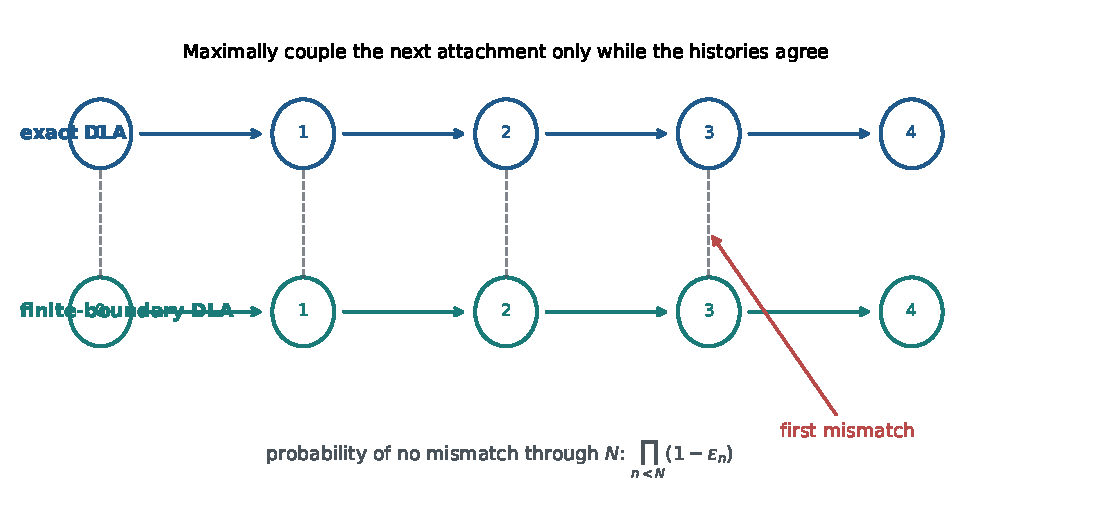
\includegraphics[width=\textwidth]{path_coupling.pdf}
  \caption{The coupling argument. It does not claim that two different DLA clusters remain geometrically close. It controls the probability of the first mismatch by coupling the next attachment only while the histories are still identical.}
  \label{fig:path-coupling}
\end{figure}

\begin{plainbox}
DLA is tip-unstable: one early difference may later change an entire branch. The proof does not deny this. Instead, it bounds the probability that any early difference occurs. Until the first mismatch, both algorithms see exactly the same cluster, so the one-step theorem can be applied again without assuming geometric stability.
\end{plainbox}

\section{Global self-centered DLA error budgets}
\label{sec:global}

At step $n$, let $Q_n$ use a measurable self-consistent center and ratio $\rho_n$. By \cref{thm:self-centered-bound}, the transition-kernel error is bounded by
\[
  \eps_n=\eps_\star(\rho_n)
  =\min\left\{1,\frac{1}{\rho_n^2(\rho_n^2-1)}\right\}.
\]

\begin{theorem}[Self-centered full-growth guarantee]
\label{thm:global-self-centered}
For every finite horizon $N$,
\begin{equation}
\boxed{
  \dTV\!\left(
  \Law(A_{n_0:N}),
  \Law(\widetilde A_{n_0:N})
  \right)
  \le
  1-\prod_{n=n_0}^{N-1}
  \left(1-\eps_\star(\rho_n)\right).
}
\label{eq:global-bound}
\end{equation}
In particular, the right-hand side is at most $\sum_n\eps_\star(\rho_n)$.
\end{theorem}

\subsection{A finite-horizon radius rule}

Suppose $M$ particles will be added using a constant ratio $\rho$ and the desired path-law budget is $\delta$. Put
\[
  \bar\eps=1-(1-\delta)^{1/M}.
\]
It is sufficient to choose
\begin{equation}
\boxed{
  \rho\ge
  \left(
  \frac{1+\sqrt{1+4/\bar\eps}}{2}
  \right)^{1/2}.
}
\label{eq:finite-radius-rule}
\end{equation}
For large $M$ and small $\delta$,
\[
  \rho\sim(M/\delta)^{1/4}.
\]

For an arbitrary center, the generic one-step bound \eqref{eq:generic-bound} requires
\[
  \rho\ge\sqrt{1+1/\bar\eps}
  \sim(M/\delta)^{1/2}.
\]
The comparison is worst-case against worst-case. Typical seed-centered clusters may have a much smaller dipole coefficient than the generic bound suggests.

\begin{figure}[H]
  \centering
  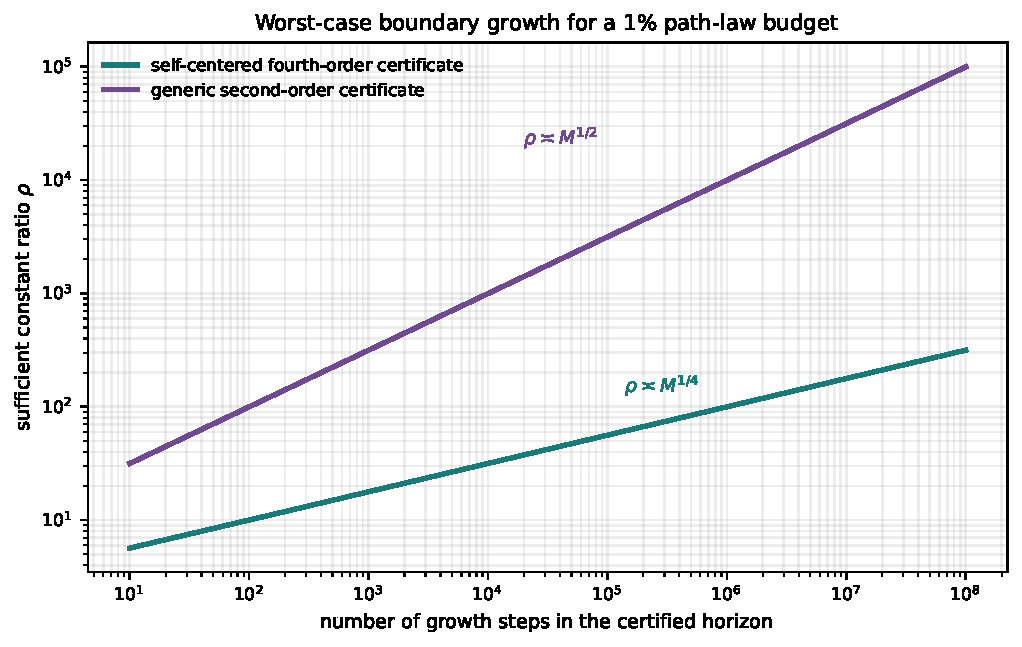
\includegraphics[width=0.86\textwidth]{global_radius_rule.pdf}
  \caption{Sufficient constant radius ratios for a $1\%$ path-space total-variation budget, using the rigorous worst-case bounds. Self-consistency changes the asymptotic requirement from square-root to fourth-root growth in the number of certified steps. These ratios are conservative and should not be read as practical recommendations without sharper constants.}
  \label{fig:global-radius}
\end{figure}

\subsection{Infinite-horizon convergence}

\begin{corollary}[Infinite path-space approximation]
\label{cor:infinite-path}
If
\[
  \sum_{n=n_0}^{\infty}\eps_\star(\rho_n)<\infty,
\]
then there is a coupling of the exact and approximate infinite histories for which
\[
  \Pp(A_n=\widetilde A_n\text{ for every }n\ge n_0)
  \ge\prod_{n=n_0}^{\infty}(1-\eps_\star(\rho_n)).
\]
The total-variation distance between the two laws on infinite path space is at most
\[
  1-\prod_{n=n_0}^{\infty}(1-\eps_\star(\rho_n))
  \le\sum_{n=n_0}^{\infty}\eps_\star(\rho_n).
\]
\end{corollary}

\begin{proof}
Apply \cref{thm:path-bound} consistently at each finite horizon. The agreement events decrease with the horizon, so continuity of probability from above gives the infinite product. The coupling inequality applies on the infinite product state space.
\end{proof}

\begin{corollary}[A sufficient one-quarter schedule]
\label{cor:quarter-threshold}
Let
\[
  \rho_n=L n^\alpha,
  \qquad L\ge\sqrt2.
\]
If $\alpha>1/4$, then
\begin{equation}
\boxed{
  \dTV\bigl(\Law(A_{n_0:\infty}),\Law(\widetilde A_{n_0:\infty})\bigr)
  \le 2L^{-4}\zeta(4\alpha,n_0)
  \le 2L^{-4}\zeta(4\alpha).
}
\label{eq:zeta-bound}
\end{equation}
Thus a target budget $\delta$ is guaranteed whenever
\[
  L\ge
  \max\left\{\sqrt2,
  \left(\frac{2\zeta(4\alpha,n_0)}{\delta}\right)^{1/4}
  \right\}.
\]
For a generic second-order center, the analogous sufficient threshold is $\alpha>1/2$.
\end{corollary}

\begin{proof}
For $\rho\ge\sqrt2$,
\[
  \frac{1}{\rho^2(\rho^2-1)}\le2\rho^{-4}.
\]
Hence $\eps_n\le2L^{-4}n^{-4\alpha}$, whose sum from the seed size is the Hurwitz tail $\zeta(4\alpha,n_0)$ and is finite when $4\alpha>1$. The generic bound is at most $2\rho^{-2}$ for $\rho\ge\sqrt2$ and therefore requires $2\alpha>1$.
\end{proof}

\begin{cautionbox}
This is a path-law budget theorem, not a claim that ordinary fixed-$\rho$ simulations converge to exact DLA as the cluster grows. With constant $\rho$, the worst-case bound is approximately $N\eps(\rho)$. The theorem says that a growing boundary schedule can make the complete path law arbitrarily accurate, and that self-consistency reduces the sufficient growth exponent from one half to one quarter.
\end{cautionbox}

\subsection{Random calibration inside the simulator}

A randomized calibration must be part of the probability model, not an informal preprocessing step. Enlarge the state at step $n$ by an auxiliary probe batch $U_n$. Conditional on the current aggregate, first sample $U_n$ from its prescribed probe kernel, compute the center as a measurable function of $(A_n,U_n)$, and then draw the actual attaching particle from a fresh random variable that is conditionally independent of $U_n$. The Ionescu--Tulcea theorem constructs the resulting joint process. This ordering ensures that a certificate proved conditionally on the realized calibration data applies to the subsequent attachment kernel.

Suppose the calibration event is good with conditional probability at least $1-\delta_n^{\mathrm{cal}}$ and, on that event, the conditional transition error is at most $\eps_n$. On the bad event, total variation is at most one. Hence the enlarged conditional kernel differs from the exact transition by at most $\eps_n+\delta_n^{\mathrm{cal}}$.

\begin{corollary}[End-to-end random-certificate budget]
\label{cor:random-calibration}
Under the enlarged-state construction above, if $\eps_n+\delta_n^{\mathrm{cal}}\le1$, then
\[
  \dTV\bigl(\Law(A_{n_0:N}),\Law(\widetilde A_{n_0:N})\bigr)
  \le1-\prod_{n=n_0}^{N-1}(1-\eps_n-\delta_n^{\mathrm{cal}}).
\]
For blockwise calibration, one charges the calibration-failure probability once at the block boundary rather than once for every attachment in that block.
\end{corollary}

\begin{proof}
On the enlarged probability space, the calibration batch is sampled first and the actual attachment uses fresh conditionally independent randomness. Conditional on the realized calibration data, the good event gives kernel error at most $\eps_n$, while the bad event contributes at most its probability $\delta_n^{\mathrm{cal}}$. Thus the unconditional one-step kernel error is at most their sum. Apply \cref{thm:path-bound} to the enlarged kernels constructed by Ionescu--Tulcea.
\end{proof}

This supplies a complete error-budget architecture. Efficiency requires the amortized construction developed next.

\section{Amortized center tracking with sublinear probe overhead}
\label{sec:amortized}

The ideal self-centered process in \cref{sec:global} is mathematically clean but computationally awkward: solving or certifying a fresh fixed point at every attachment requires too many frozen-cluster probes. This section replaces exact per-step self-consistency by two cheaper operations:

\begin{enumerate}
  \item one empirical barycenter update at the start of a block; and
  \item reuse of that center while a controlled number of particles are added.
\end{enumerate}

The new ingredient is a deterministic bound on how quickly the true harmonic-measure barycenter can move under bounded disk growth.

\subsection{Diameter-scaled boundaries and one-shot recentering}

For tracking, it is convenient to make the death radius independent of the trial center. Write
\[
  D(K)=\operatorname{diam}K,
  \qquad
  h_K=\int_K z\,\omega_K(\dd z),
\]
and, for $c\in\conv(K)$, define
\begin{equation}
  \bar\nu_{\varrho,c}^{K}=\nu_{d,c},
  \qquad d=\varrho D(K),
  \qquad
  \bar\Phi_{\varrho}^{K}(c)=\int_K z\,\bar\nu_{\varrho,c}^{K}(\dd z).
  \label{eq:diameter-law}
\end{equation}
Because $c\in\conv(K)$, every $z\in K$ satisfies $|z-c|\le D(K)$, so the death disk contains the target whenever $\varrho>1$.

\begin{proposition}[Diameter-scaled residual and one-shot recentering]
\label{prop:one-shot}
Let $K$ be compact and nonpolar, let $D=D(K)>0$, and let $\varrho>1$.

For every $c\in\conv(K)$,
\begin{align}
  \dTV\!\left(\bar\nu_{\varrho,c}^{K},\omega_K\right)
  &\le
  \min\left\{1,
  \varrho^{-2}\frac{|\bar\Phi_{\varrho}^{K}(c)-c|}{D}
  +\frac{1}{\varrho^2(\varrho^2-1)}\right\},
  \label{eq:diameter-residual}
  \\
  \frac{|\bar\Phi_{\varrho}^{K}(c)-h_K|}{D}
  &\le \frac{2}{\varrho^2-1}.
  \label{eq:finite-barycenter-close}
\end{align}

Now draw $M$ independent points $Y_1,\ldots,Y_M$ with law
$\bar\nu_{\varrho,c}^{K}$ and put
\[
  c^+=\frac1M\sum_{j=1}^{M}Y_j.
\]
For every $\chi\in(0,1)$, with probability at least $1-\chi$,
\begin{align}
  \frac{|c^+-h_K|}{D}
  &\le
  2\sqrt{\frac{\log(4/\chi)}{M}}
  +\frac{2}{\varrho^2-1},
  \label{eq:one-shot-center}
  \\
  \dTV\!\left(\bar\nu_{\varrho,c^+}^{K},\omega_K\right)
  &\le
  2\varrho^{-2}\sqrt{\frac{\log(4/\chi)}{M}}
  +\frac{5}{\varrho^2(\varrho^2-1)},
  \label{eq:one-shot-law}
\end{align}
with the last right-hand side capped at one.
\end{proposition}

\begin{proof}
The first claim follows from \cref{prop:residual-bounds} because
$R_K(c)\le D$ and $d=\varrho D$. The generic bound similarly gives
\[
  \dTV(\bar\nu_{\varrho,c}^{K},\omega_K)
  \le \min\{1,(\varrho^2-1)^{-1}\}.
\]
Both measures have mass one, so centering the coordinate function at any point of $\conv(K)$ gives
\[
  |\bar\Phi_{\varrho}^{K}(c)-h_K|
  \le D\norm{\bar\nu_{\varrho,c}^{K}-\omega_K}_{\mathrm{var}},
\]
which proves \eqref{eq:finite-barycenter-close}.

Each coordinate of $Y_j-c$ lies in an interval of length at most $2D$.
Hoeffding's inequality and a two-coordinate union bound give
\[
  |c^+-\bar\Phi_{\varrho}^{K}(c)|
  \le 2D\sqrt{\frac{\log(4/\chi)}{M}}
\]
with probability at least $1-\chi$. This and
\eqref{eq:finite-barycenter-close} prove \eqref{eq:one-shot-center}.
Finally,
\[
  |\bar\Phi_{\varrho}^{K}(c^+)-c^+|
  \le
  |\bar\Phi_{\varrho}^{K}(c^+)-h_K|+|h_K-c^+|.
\]
Use \eqref{eq:finite-barycenter-close} once more and substitute the
resulting residual into \eqref{eq:diameter-residual}.
\end{proof}

\begin{plainbox}
A fixed-point solver is not needed to recover fourth-order accuracy. Start from any center inside the convex hull, estimate the approximate attachment mean once, and use that mean as the new center. The first estimate is already within second-order distance of the true growth-probability center; multiplying that displacement by the second-order dipole factor makes the resulting attachment-law error fourth order.
\end{plainbox}

\subsection{How far can the harmonic center move in one growth step?}
\label{sec:center-drift}

The results in this subsection are independent of the restart algorithm. In particular, \cref{lem:nested-centers,thm:center-drift} give explicit continuity estimates for conformal centers of nested planar continua under bounded parallel enlargement, and may be useful outside DLA simulation. They sit beside classical kernel-convergence theory for conformal maps and more recent work on capacity continuity under Hausdorff perturbation \cite{Pommerenke1992,KalmykovKovalev2022}; we have not found the explicit nested-center inequality \eqref{eq:nested-center-bound} in that literature.

We now impose only geometric assumptions satisfied by ordinary bounded-radius disk aggregation.

\begin{assumption}[Bounded disk-growth geometry]
\label{ass:disk-growth}
There are constants $a_0>0$ and $\delta_0>0$ such that the capture targets
$K_n$ satisfy:
\begin{enumerate}
  \item $K_n\subset K_{n+1}$ and each $K_n$ is a connected compact set;
  \item $K_n$ contains $n$ pairwise interior-disjoint disks of radius $a_0$;
  \item $K_{n+1}\subset (K_n)_{\delta_0}
  :=\{z:\operatorname{dist}(z,K_n)\le\delta_0\}$.
\end{enumerate}
\end{assumption}

For equal physical particles, the disjoint disks in item 2 are the particles themselves. Item 3 merely says that one attachment changes the target only within a fixed Euclidean distance of the existing target. The constants allow the physical-particle radius and the capture radius to differ.

For a connected compact set $K$, let
\[
  r_K=\caplog(K),
  \qquad
  h_K=\int_Kz\,\omega_K(\dd z).
\]
For the full hull of $K$, the normalized exterior map has expansion
$F(w)=r_Kw+h_K+O(w^{-1})$: harmonic measure from infinity is the pushforward of uniform angular measure, so the constant Laurent coefficient is exactly the harmonic-measure barycenter. Filling bounded complementary components does not change $r_K$, $h_K$, or the diameter, and the following conformal arguments may therefore be applied to the polynomial hull of $K$.

\begin{lemma}[Capacity of a parallel neighborhood]
\label{lem:parallel-capacity}
Let $K$ be a continuum of logarithmic capacity $r>0$ and let
$K_\delta=\{z:\operatorname{dist}(z,K)\le\delta\}$. Put $u=\delta/r$ and
\[
  S(u)=1+\frac{u}{2}+\frac12\sqrt{u^2+4u}.
\]
Then
\begin{equation}
  \caplog(K_\delta)\le rS(u).
  \label{eq:parallel-capacity}
\end{equation}
If $0<u\le1$, then
\begin{equation}
  S(u)^2-1\le6\sqrt{u}.
  \label{eq:S-bound}
\end{equation}
\end{lemma}

\begin{proof}
Replace $K$ by its full hull. Since the original $K_\delta$ is contained in the $\delta$-neighborhood of that hull, this can only increase the capacity that must be bounded. Let
\[
  F(w)=rw+h+a_1w^{-1}+\cdots,
  \qquad |w|>1,
\]
map the exterior unit disk conformally onto $\widehat\C\setminus K$.
For any $a\in K$, the function
\[
  g_a(\zeta)=\frac{r}{F(1/\zeta)-a}
\]
extends to a normalized univalent map of the unit disk. The Koebe growth theorem therefore yields \cite{Pommerenke1992}
\[
  |F(w)-a|\ge r\frac{(|w|-1)^2}{|w|}.
\]
Taking the infimum over $a\in K$ gives the same lower bound for
$\operatorname{dist}(F(w),K)$. Hence every point within distance $\delta$
of $K$ has preimage modulus at most the larger root of
$(t-1)^2/t=u$, namely $S(u)$. It follows that $K_\delta$ is contained in
the compact set whose exterior map is $w\mapsto F(S(u)w)$; that compact
set has capacity $rS(u)$.

For $u=x^2\le1$,
\[
  S(u)-1\le\frac{1+\sqrt5}{2}x,
  \qquad
  S(u)+1\le2+\frac{1+\sqrt5}{2},
\]
and the product is less than $6x$.
\end{proof}

\begin{lemma}[Nested conformal centers]
\label{lem:nested-centers}
Let $K\subset K'$ be full continua with capacities $r\le r'$ and harmonic centers $h,h'$. Then
\begin{equation}
  |h'-h|\le\frac{r'^2-r^2}{r}.
  \label{eq:nested-center-bound}
\end{equation}
\end{lemma}

\begin{proof}
Let $F,F'$ be the normalized exterior maps of $K,K'$. Since the exterior
of $K'$ is contained in the exterior of $K$,
\[
  \psi=F^{-1}\circ F'
\]
maps $|w|>1$ into itself and has expansion
\[
  \psi(w)=\lambda w+b+O(w^{-1}),
  \qquad
  \lambda=\frac{r'}{r},
  \qquad
  b=\frac{h'-h}{r}.
\]
The function $f(z)=1/\psi(1/z)$ maps the unit disk into itself, fixes zero,
and satisfies
\[
  \frac{f(z)}{z}=\lambda^{-1}-b\lambda^{-2}z+O(z^2).
\]
Schwarz--Pick applied to $f(z)/z$ at zero gives
$|b|/\lambda^2\le1-\lambda^{-2}$, hence
$|b|\le\lambda^2-1$. Multiplying by $r$ proves
\eqref{eq:nested-center-bound}.
\end{proof}

\begin{theorem}[Deterministic harmonic-center drift]
\label{thm:center-drift}
Under \cref{ass:disk-growth}, put
\[
  D_n=\operatorname{diam}K_n,
  \qquad
  h_n=\int_{K_n}z\,\omega_{K_n}(\dd z),
  \qquad
  C_{\mathrm{drift}}=3\sqrt{\frac{\delta_0}{a_0}}.
\]
For every $n$ with $4\delta_0/D_n\le1$,
\begin{equation}
\boxed{
  \frac{|h_{n+1}-h_n|}{D_n}
  \le 3\sqrt{2}\,\sqrt{\frac{\delta_0}{D_n}}
  \le C_{\mathrm{drift}}\,n^{-1/4}.
}
\label{eq:center-drift}
\end{equation}
In particular, the condition holds for every
\begin{equation}
  n\ge n_{\mathrm{geom}}
  :=\left\lceil\frac{4\delta_0^2}{a_0^2}\right\rceil.
  \label{eq:n-geom}
\end{equation}
\end{theorem}

\begin{proof}
Let $H_n$ be the polynomial hull of $K_n$, and write $r_n=\caplog(K_n)$.
The hulls are nested and have the same capacities, harmonic centers, and
diameters as the original targets. By monotonicity and
$K_{n+1}\subset(K_n)_{\delta_0}\subset(H_n)_{\delta_0}$,
\[
  r_{n+1}\le\caplog((H_n)_{\delta_0}).
\]
Apply \cref{lem:parallel-capacity,lem:nested-centers} with
$u=\delta_0/r_n$. For continua of diameter $D_n$, the classical
P\'olya--Szeg\H{o} bounds give
\[
  \frac{D_n}{4}\le r_n\le\frac{D_n}{2}
  \qquad\text{\cite{PolyaSzego1951}}.
\]
When $u\le1$, \eqref{eq:S-bound} therefore yields
\[
  \frac{|h_{n+1}-h_n|}{D_n}
  \le\frac{r_n}{D_n}\bigl(S(u)^2-1\bigr)
  \le 6\frac{\sqrt{\delta_0r_n}}{D_n}
  \le3\sqrt{2}\sqrt{\frac{\delta_0}{D_n}}.
\]
Finally, the $n$ disjoint radius-$a_0$ disks have total area
$n\pi a_0^2$. The planar isodiametric inequality gives
$D_n\ge2a_0\sqrt n$, and hence the last term is at most
$3\sqrt{\delta_0/a_0}\,n^{-1/4}$. The explicit condition
$n\ge n_{\mathrm{geom}}$ follows from
$4\delta_0/(2a_0\sqrt n)\le1$.
\end{proof}

\begin{corollary}[Diameter-growth refinement]
\label{cor:diameter-growth-drift}
Suppose, in addition to \cref{ass:disk-growth}, that for some constants
$c_D>0$, $\xi\ge1/2$, and $n_1$,
\[
  D_n\ge c_D n^\xi,
  \qquad n\ge n_1.
\]
Then, whenever $4\delta_0/D_n\le1$,
\begin{equation}
  \frac{|h_{n+1}-h_n|}{D_n}
  \le C_\xi n^{-\xi/2},
  \qquad
  C_\xi=3\sqrt{\frac{2\delta_0}{c_D}}.
  \label{eq:diameter-refined-drift}
\end{equation}
The hypothesis is directly checkable along a simulated trajectory. It does not assume a fractal dimension; it merely records any verified lower growth rate of the observed diameter.
\end{corollary}

\begin{proof}
Substitute $D_n\ge c_Dn^\xi$ into the first inequality in
\eqref{eq:center-drift}.
\end{proof}

\begin{plainbox}
One new particle can alter which tips are exposed, but it cannot move the growth-probability center by an arbitrary fraction of the whole cluster diameter. Capacity and conformal distortion force the normalized movement to be at most a constant times $n^{-1/4}$. This worst-case estimate is exactly what permits a center to be reused for a growing block of attachments.
\end{plainbox}

\begin{figure}[H]
  \centering
  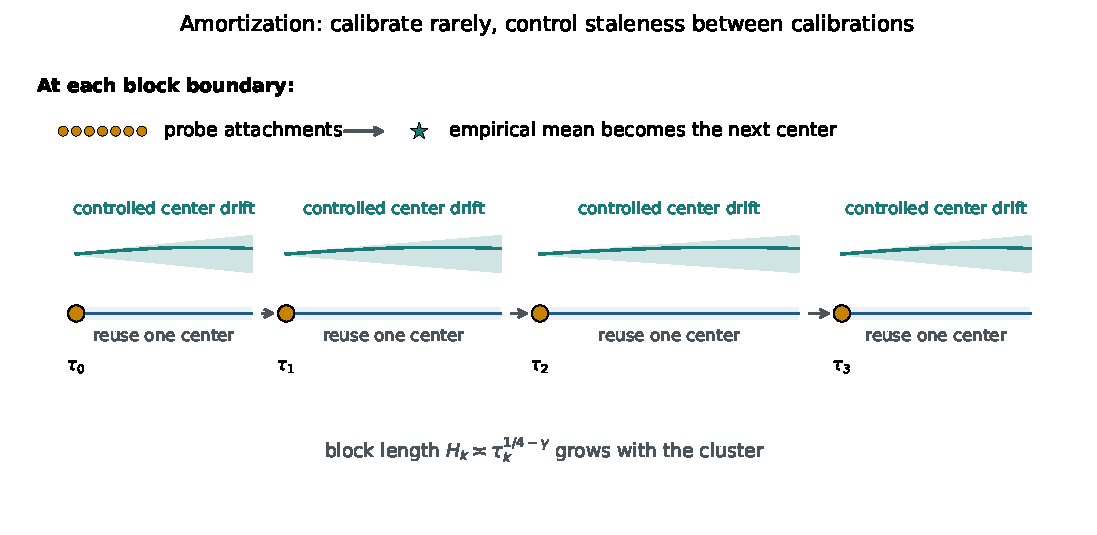
\includegraphics[width=\textwidth]{amortized_schedule.pdf}
  \caption{Blockwise center tracking. Frozen-cluster probes are used only at block boundaries. Within a block, the calibrated center is held fixed; the deterministic drift theorem bounds how stale it can become before the next recalibration.}
  \label{fig:amortized-schedule}
\end{figure}

\subsection{The blockwise algorithm}

Choose exponents $\alpha,\gamma>0$ and set
\begin{equation}
  \varrho_n=Ln^\alpha,
  \qquad
  \kappa=\frac14-\gamma.
  \label{eq:amortized-parameters}
\end{equation}
Starting from an integer
\[
  \tau_0\ge
  \max\left\{n_{\mathrm{geom}},\left\lceil2^{1/\kappa}\right\rceil\right\},
\]
define calibration times by
\begin{equation}
  \tau_{k+1}=\tau_k+H_k,
  \qquad
  H_k=\left\lfloor\tau_k^\kappa\right\rfloor.
  \label{eq:block-times}
\end{equation}
At time $\tau_k$:

\begin{enumerate}
  \item choose any measurable pilot point $p_k\in\conv(K_{\tau_k})$;
  \item draw $M_k$ independent frozen-cluster probes from
  $\bar\nu_{\varrho_{\tau_k},p_k}^{K_{\tau_k}}$;
  \item set $c_k$ equal to their empirical mean;
  \item for each $n\in[\tau_k,\tau_{k+1})$, draw the actual attaching particle independently from
  $\bar\nu_{\varrho_n,c_k}^{K_n}$.
\end{enumerate}

The previous block center is an admissible pilot because the convex hulls are nested. No iterative fixed-point search is required.

\begin{algorithm}[H]
\caption{Amortized center tracking}
\label{alg:amortized}
\begin{algorithmic}[1]
\State Choose $L,\alpha,\gamma$, failure probabilities $(\delta_k)$, and $\tau_0\ge\max\{n_{\mathrm{geom}},\lceil2^{1/\kappa}\rceil\}$
\For{$k=0,1,2,\ldots$}
  \State $H_k\gets\lfloor\tau_k^{1/4-\gamma}\rfloor$
  \State $M_k\gets\left\lceil4\tau_k^{2\gamma}\log(4/\delta_k)\right\rceil$
  \State Draw $M_k$ frozen-cluster probes at $K_{\tau_k}$ from a pilot center $p_k$
  \State $c_k\gets$ empirical mean of the probe attachment points
  \For{$n=\tau_k,\ldots,\tau_k+H_k-1$}
    \State attach one fresh walker using center $c_k$ and death radius $Ln^\alpha D_n$
  \EndFor
  \State $\tau_{k+1}\gets\tau_k+H_k$
\EndFor
\end{algorithmic}
\end{algorithm}

\subsection{The amortized path-space theorem}

\begin{theorem}[Sublinear-overhead amortized center tracking]
\label{thm:amortized}
Assume \cref{ass:disk-growth}. Let
\[
  \alpha>\frac{11}{24},
  \qquad
  \max\{0,1-2\alpha\}<\gamma<\frac1{12},
  \qquad
  \kappa=\frac14-\gamma,
  \qquad
  L\ge\sqrt2.
\]
Choose
\[
  \tau_0\ge
  \max\left\{n_{\mathrm{geom}},\left\lceil2^{1/\kappa}\right\rceil\right\}.
\]
Then $\tau_k^\kappa\ge2$ for every block, so $H_k\ge\tau_k^\kappa/2$ and $\tau_{k+1}\le2\tau_k$ from the first block onward. Run \cref{alg:amortized} with the minimal certified batch sizes
\begin{equation}
  M_k=
  \left\lceil4\tau_k^{2\gamma}\log(4/\delta_k)\right\rceil,
  \qquad
  \sum_{k\ge0}\delta_k\le\delta_{\mathrm{cal}}.
  \label{eq:batch-size}
\end{equation}
Then there are constants
\begin{equation}
  C_1=2^\gamma(1+C_{\mathrm{drift}}),
  \qquad
  C_2=2^{2\alpha+2}+6,
  \label{eq:amortized-constants}
\end{equation}
depending only on the displayed parameters and the disk-growth geometry, such that, when the exact and amortized processes share the same target at time $\tau_0$, their infinite histories from that time onward satisfy
\begin{equation}
\boxed{
  \dTV\bigl(\Law(A_\bullet),\Law(\widetilde A_\bullet)\bigr)
  \le
  \delta_{\mathrm{cal}}
  +C_1L^{-2}\zeta(2\alpha+\gamma,\tau_0)
  +C_2L^{-4}\zeta(4\alpha,\tau_0).
}
\label{eq:amortized-path-bound}
\end{equation}
Here $\zeta(s,a)=\sum_{j=0}^{\infty}(a+j)^{-s}$ is the Hurwitz zeta function. Replacing the two Hurwitz tails by the larger Riemann-zeta values gives a simpler bound independent of $\tau_0$.

If, for example,
\begin{equation}
  \delta_k=\frac{6\delta_{\mathrm{cal}}}{\pi^2(k+1)^2},
  \label{eq:failure-schedule}
\end{equation}
then the total number $P_N$ of frozen-cluster probes used through size $N$ obeys
\begin{equation}
\boxed{
  P_N
  =O\!\left(
    N^{3/4+3\gamma}
    \log\frac{N}{\delta_{\mathrm{cal}}}
  \right)
  =o(N).
}
\label{eq:sublinear-probes}
\end{equation}
Consequently, for every target path-space budget $\delta>0$, one can first choose $\delta_{\mathrm{cal}}<\delta$ and then choose $L$ sufficiently large so that the right-hand side of \eqref{eq:amortized-path-bound} is at most $\delta$, while retaining sublinear probe count.
\end{theorem}

\begin{proof}
At calibration time $\tau_k$, \cref{prop:one-shot} and
\eqref{eq:batch-size} give, except on an event of conditional probability
at most $\delta_k$,
\begin{equation}
  \frac{|c_k-h_{\tau_k}|}{D_{\tau_k}}
  \le \tau_k^{-\gamma}
  +\frac{2}{\varrho_{\tau_k}^2-1}.
  \label{eq:block-initial-center}
\end{equation}
For $n\in[\tau_k,\tau_{k+1})$, diameter monotonicity and
\cref{thm:center-drift} imply
\begin{equation}
  \frac{|h_n-h_{\tau_k}|}{D_n}
  \le C_{\mathrm{drift}}H_k\tau_k^{-1/4}
  \le C_{\mathrm{drift}}\tau_k^{-\gamma}.
  \label{eq:block-drift}
\end{equation}
For the current finite-boundary barycenter, the generic estimate
\eqref{eq:finite-barycenter-close} gives
\[
  \frac{|\bar\Phi_{\varrho_n}^{K_n}(c_k)-h_n|}{D_n}
  \le\frac{2}{\varrho_n^2-1}.
\]
Combining the last three displays and using $D_{\tau_k}\le D_n$ yields
\begin{equation}
  \frac{|\bar\Phi_{\varrho_n}^{K_n}(c_k)-c_k|}{D_n}
  \le
  (1+C_{\mathrm{drift}})\tau_k^{-\gamma}
  +\frac{2}{\varrho_{\tau_k}^2-1}
  +\frac{2}{\varrho_n^2-1}.
  \label{eq:stale-residual}
\end{equation}
Since $H_k\le\tau_k^\kappa\le\tau_k$, one has $n\le2\tau_k$.
With $\varrho_j=Lj^\alpha$ and $L\ge\sqrt2$, substitution into
\eqref{eq:diameter-residual} gives the conditional one-step bound
\begin{equation}
  \dTV(P_n,Q_n)
  \le
  C_1L^{-2}n^{-(2\alpha+\gamma)}
  +C_2L^{-4}n^{-4\alpha}
  =:\varepsilon_n.
  \label{eq:amortized-local}
\end{equation}
The two exponents exceed one by the assumptions on $\alpha$ and $\gamma$.

Construct the process on an enlarged probability space. At each block
boundary, conditional on the current aggregate, first draw the frozen-cluster
probe batch, compute $c_k$ as a measurable function of that batch, and only
then draw every growth attachment in the block from fresh randomness.
The Ionescu--Tulcea construction and \cref{lem:maximal-kernel-coupling}
therefore apply to the resulting conditional kernels. Declare a coupling
failure whenever a calibration event fails, and otherwise use maximal
coupling for the actual attachments while the histories agree. The total
failure probability is at most
\[
  \sum_k\delta_k+\sum_n\varepsilon_n,
\]
which proves \eqref{eq:amortized-path-bound}.

It remains to count probes. For all sufficiently large $\tau_k$,
$H_k\ge\tau_k^\kappa/2$ and $\tau_{k+1}\le2\tau_k$. Applying the mean-value theorem to $x^{1-\kappa}$ gives a positive constant lower bound on
$\tau_{k+1}^{1-\kappa}-\tau_k^{1-\kappa}$. Consequently,
\[
  \#\{k:\tau_k\le N\}=O(N^{1-\kappa}).
\]
Under \eqref{eq:failure-schedule},
$\log(4/\delta_k)=O(\log(N/\delta_{\mathrm{cal}}))$ for every block before $N$.
Therefore
\[
  P_N
  \le
  O(N^{1-\kappa})\,
  O(N^{2\gamma})\,
  O\!\left(\log\frac{N}{\delta_{\mathrm{cal}}}\right),
\]
and $1-\kappa+2\gamma=3/4+3\gamma<1$.
\end{proof}

\begin{corollary}[Including the finite prefix]
\label{cor:exact-prefix}
Start from the prescribed seed of size $n_0$. If exact Poisson return is used for the finite prefix $n_0\le n<\tau_0$ and the amortized scheme is used thereafter, then the bound in \eqref{eq:amortized-path-bound} applies to the complete history from the seed. More generally, if an approximate prefix has an independently established path-space budget $\delta_{\mathrm{pre}}$, then $\delta_{\mathrm{pre}}$ is added to the right-hand side of \eqref{eq:amortized-path-bound}.
\end{corollary}

\begin{proof}
Under an exact prefix the two coupled histories are identical at time $\tau_0$, so \cref{thm:amortized} applies directly. For an approximate prefix, couple the prefix first and then condition on agreement at $\tau_0$; the union bound, or the product form in \cref{thm:path-bound}, gives the additive statement.
\end{proof}

\begin{corollary}[Diameter-adaptive exponent improvement]
\label{cor:diameter-adaptive-amortization}
Assume the hypotheses of \cref{cor:diameter-growth-drift} and suppose the verified lower bound $D_n\ge c_Dn^\xi$ holds throughout the calibrated regime. Replace the block exponent in \eqref{eq:amortized-parameters} by
\[
  \kappa=\frac{\xi}{2}-\gamma.
\]
If
\[
  \alpha>\frac12-\frac{\xi}{12},
  \qquad
  \max\{0,1-2\alpha\}<\gamma<\frac{\xi}{6},
\]
then the proof of \cref{thm:amortized} gives a finite bound on the infinite-horizon path distance and
\begin{equation}
  P_N=O\!\left(
    N^{1-\xi/2+3\gamma}
    \log\frac{N}{\delta_{\mathrm{cal}}}
  \right)=o(N).
  \label{eq:diameter-adaptive-probes}
\end{equation}
Thus any runtime-verified diameter growth faster than the area-only exponent $1/2$ improves the sufficient boundary threshold below $11/24$.
\end{corollary}

\begin{proof}
By \cref{cor:diameter-growth-drift}, normalized center drift is
$O(n^{-\xi/2})$. A block of length $n^{\xi/2-\gamma}$ therefore accumulates $O(n^{-\gamma})$ staleness. The stale dipole remains summable when $2\alpha+\gamma>1$. The number of blocks through $N$ is $O(N^{1-\xi/2+\gamma})$, and each calibration uses $O(N^{2\gamma}\log(N/\delta_{\mathrm{cal}}))$ probes, giving \eqref{eq:diameter-adaptive-probes}. Sublinearity is equivalent to $3\gamma<\xi/2$. A feasible $\gamma$ exists exactly when $1-2\alpha<\xi/6$, which is the displayed condition on $\alpha$.
\end{proof}

\begin{figure}[H]
  \centering
  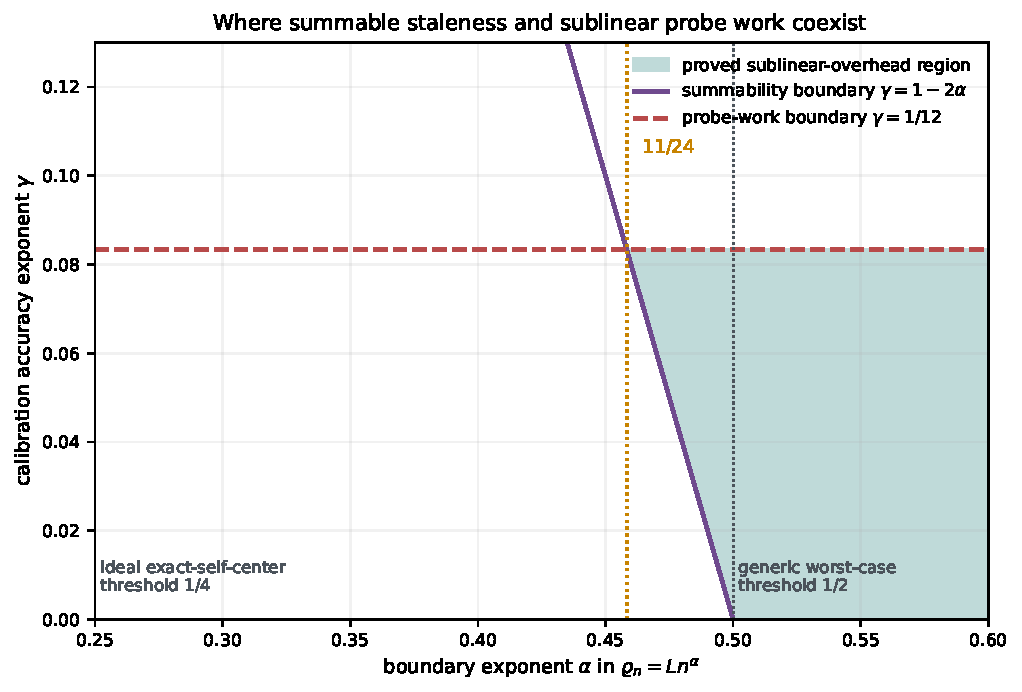
\includegraphics[width=0.84\textwidth]{amortized_feasible_region.pdf}
  \caption{Exponent region for the proved blockwise architecture under the area-only diameter bound $\xi=1/2$. Summable stale-center error requires $2\alpha+\gamma>1$, while sublinear probe count requires $\gamma<1/12$; their intersection begins at $\alpha>11/24$. If a runtime-verified bound $D_n\ge c_Dn^\xi$ holds with $\xi>1/2$, \cref{cor:diameter-adaptive-amortization} shifts the feasible region downward to the sufficient threshold $\alpha>1/2-\xi/12$. The ideal exact-self-center threshold remains $1/4$, while the generic uncentered worst-case threshold is $1/2$.}
  \label{fig:amortized-region}
\end{figure}

\begin{corollary}[Sublinear weighted calibration work]
\label{cor:weighted-work}
Let $W_n$ be a nondecreasing reference cost satisfying
$W_{2n}\le C_WW_n$. Suppose the expected cost of one frozen-cluster probe at
size $n$ is at most $C_pW_n$, while the expected cost of one ordinary growth
walker is at least $c_gW_n$, for constants $C_p,c_g>0$. Then the ratio of
expected calibration work through size $N$ to the expected work of the $N$
ordinary growth walkers is
\begin{equation}
  O\!\left(
  N^{-1/4+3\gamma}
  \log\frac{N}{\delta_{\mathrm{cal}}}
  \right)=o(1).
  \label{eq:weighted-overhead}
\end{equation}
\end{corollary}

\begin{proof}
The calibration work is at most $C_pP_NW_N$. The growth work over the final
half of the horizon is at least
\[
  c_g(N/2)W_{\lfloor N/2\rfloor}
  \ge \frac{c_gN}{2C_W}W_N.
\]
Apply \eqref{eq:sublinear-probes}.
\end{proof}

\begin{remark}[Interpretation of the cost model]
The doubling condition on $W_n$ is an explicit modeling assumption, not a consequence of the probability theorem. Although the absolute death radius grows with both cluster size and $\varrho_n$, walk-on-spheres crosses successively larger empty scales in only logarithmically many idealized jumps; moreover, the probability of repeated outer excursions falls as the boundary is moved outward. This makes a doubling model plausible \cite{Muller1956}, but it must be checked for the actual spatial index, collision test, and restart implementation used in software. The probe-count theorem \eqref{eq:sublinear-probes} does not depend on this assumption; only the conversion from probe count to wall-clock work does.
\end{remark}

\begin{costbox}
The theorem closes the specific worst-case staleness problem raised by per-step certification. It reduces extra probe count from roughly quadratic to sublinear and, under a mild doubling model, makes probe work negligible relative to the baseline sequence of growth walkers. The price is a more conservative boundary exponent: the proved amortized schedule requires $\alpha>11/24\approx0.4583$, rather than the ideal exact-self-center threshold $\alpha>1/4$. It still improves on the generic worst-case requirement $\alpha>1/2$.
\end{costbox}

\begin{remark}[Why $11/24$ appears]
Within this particular blockwise Hoeffding architecture, the sufficient exponent constraints derived below meet at $11/24$. Sampling the center to normalized accuracy $n^{-\gamma}$ costs $n^{2\gamma}$ probes. The drift theorem permits blocks of length at most $n^{1/4-\gamma}$. Hence total probe count is sublinear only when $3\gamma<1/4$. Summability of the stale dipole requires $2\alpha+\gamma>1$. Letting $\gamma$ approach $1/12$ gives $\alpha>11/24$. This is not a universal lower bound: sharper probabilistic center drift, variance-sensitive estimation, or reuse of ordinary growth attachments could improve it.
\end{remark}


\section{Computational meaning and honest cost comparison}

\subsection{Exact return is the practical baseline}

For concentric circular boundaries, exact return uses the Poisson kernel and is unbiased. It requires retaining the escape angle and sampling one return angle; the boundary correction itself is $O(1)$ work per escape. It also avoids estimating a center. Therefore a self-centered uniform-restart method should not be advertised as faster without benchmark evidence.

The theory is most directly useful for:

\begin{itemize}
  \item explaining and certifying legacy uniform-restart codes;
  \item validating approximate return rules;
  \item hardware settings where branch-free uniform relaunch is attractive;
  \item and theoretical studies that require an explicit path-space error budget.
\end{itemize}

Every theorem in this manuscript uses a circular death boundary. For a noncircular boundary, the return kernel is no longer diagonal in Fourier modes and the identity \eqref{eq:exact-weak} must be replaced by a boundary-operator expansion. Such an extension may be possible, but it is not established here and is not part of the practical motivation claimed by this paper.

\subsection{From quadratic certification to sublinear tracking}

To keep the per-step Hoeffding term in \eqref{eq:mc-certificate} at fourth-order scale, a fresh calibration requires
\[
  M_n\gtrsim \varrho_n^4\log(1/\delta_n^{\mathrm{cal}})
\]
probes. Under $\varrho_n=Ln^\alpha$, recalibrating independently after every attachment costs at least
\[
  \sum_{n\le N}M_n\gtrsim N^{4\alpha+1}\log N,
\]
which is roughly quadratic near the ideal threshold $\alpha=1/4$.

\Cref{thm:amortized} changes that conclusion for bounded disk growth. Its blockwise method needs only
\[
  O\!\left(N^{3/4+3\gamma}\log(N/\delta_{\mathrm{cal}})\right)=o(N)
\]
frozen-cluster probes, and \cref{cor:weighted-work} makes their work asymptotically negligible under a mild doubling model. The improvement comes from three facts:

\begin{enumerate}
  \item a single barycenter update already restores fourth-order one-step accuracy;
  \item the true harmonic center has normalized drift at most $O(n^{-1/4})$;
  \item a center can therefore be reused over a block of length $n^{1/4-\gamma}$.
\end{enumerate}

\begin{costbox}
The amortized theorem resolves the previous worst-case staleness objection at the level of additional probe count. It does not prove that a Python or C implementation beats exact Poisson return in wall-clock time. The certified schedule uses larger death-radius growth than the ideal fixed-point theorem, and practical performance still depends on spatial indexing, walk-on-spheres cost, memory traffic, vectorization, and constants hidden by the asymptotic bounds.
\end{costbox}

The principal algorithmic questions are now sharper: can ordinary growth attachments be reused as center data without bias; can the deterministic $n^{-1/4}$ drift be improved to a typical DLA rate; can variance-sensitive confidence sequences replace Hoeffding; and can the boundary exponent be driven from $11/24$ toward the ideal $1/4$ while preserving sublinear overhead?

\section{Smooth-boundary multipole asymptotics}
\label{sec:smooth-asymptotics}

The preceding compact-set results are the ones relevant to actual finite disk-union DLA targets. Under additional smoothness, one can say more: the first nonzero equilibrium moment determines an exact asymptotic power and a nonzero leading coefficient in density norm.

Let $K$ have a $C^{2,\sigma}$ Jordan boundary $\Gamma$, fix a center $c$, write $R=R_K(c)$ and $\rho=d/R$, and define normalized moments
\[
  \mathcal M_n(c;\mu)=R^{-n}M_n^c(\mu).
\]

The disk Green kernel is
\begin{equation}
  g_{d,c}(z,w)=
  \log\left|
  \frac{d^2-(z-c)\overline{(w-c)}}{d(z-w)}
  \right|.
  \label{eq:disk-green}
\end{equation}
For every probability measure $\mu$ on $K$,
\begin{equation}
  I_{d,c}(\mu)
  =\log d+I_\infty(\mu)
  -\sum_{n=1}^{\infty}
   \frac{\rho^{-2n}}{n}
   |\mathcal M_n(c;\mu)|^2.
  \label{eq:energy-expansion}
\end{equation}
The series is exact and uniformly absolutely convergent.

\begin{lemma}[Regularity and identification of the smooth equilibrium density]
\label{lem:smooth-density}
For every sufficiently large $\rho$, the Green equilibrium measure of $K$ relative to $D(c,\rho R)$ is supported on all of $\Gamma$ and has a strictly positive $C^{0,\sigma}(\Gamma)$ density. This density, together with its equilibrium-potential constant, is the unique solution in $C^{0,\sigma}(\Gamma)\times\mathbb R$ of the augmented boundary integral equation used below.
\end{lemma}

\begin{proof}
Let $v_\rho$ be the condenser potential equal to one on $\Gamma$ and zero on the outer circle. Schauder boundary regularity for the Dirichlet problem on a $C^{2,\sigma}$ boundary gives $v_\rho\in C^{1,\sigma}$ up to $\Gamma$. The Hopf boundary lemma shows that its inward normal derivative is strictly positive at every point of $\Gamma$. The normalized flux $\partial_n v_\rho\,\dd s$ is therefore a strictly positive $C^{0,\sigma}$ density and is the Green equilibrium measure. Its Green potential is constant on $\Gamma$, so it solves the augmented integral equation. Conversely, any mass-one density solving that equation has constant Green potential on $\Gamma$ and hence, by uniqueness of the Green equilibrium measure, equals the normalized condenser flux. Uniqueness of the augmented equation follows for all sufficiently large $\rho$ from the invertibility at $\rho=\infty$ and a small-norm perturbation argument.
\end{proof}

\begin{theorem}[Smooth-boundary moment asymptotics]
\label{thm:smooth-asymptotic}
Suppose
\[
  \mathcal M_1(c;\omega_K)=\cdots=
  \mathcal M_{m-1}(c;\omega_K)=0,
  \qquad
  \mathcal M_m(c;\omega_K)\ne0.
\]
Then there is a nonzero real signed measure $\Lambda_m$, of total mass zero and with a $C^{0,\sigma}$ density, such that
\[
  \nu_{d,c}-\omega_K
  =\rho^{-2m}\Lambda_m
  +O_{C^{0,\sigma}}(\rho^{-2m-2}).
\]
Consequently,
\[
  \dTV(\nu_{d,c},\omega_K)
  =C_m\rho^{-2m}+O(\rho^{-2m-2}),
  \qquad C_m>0.
\]
\end{theorem}

\begin{proof}
Put $t=\rho^{-2}$. On $C^{0,\sigma}(\Gamma)\times\mathbb R$, define
\[
  \mathcal A_t(\sigma,V)
  =\left(
  S\sigma-V
  -\sum_{n\ge1}\frac{t^n}{n}
  \Real\left[\widehat z^{\,n}
  \overline{\mathcal M_n(c;\sigma)}\right],
  \int_\Gamma\sigma\dd s
  \right).
\]
The unperturbed operator $\mathcal A_0$ is an isomorphism on the relevant H\"older spaces \cite{Kress2014}. The perturbation series converges in operator norm for $|t|$ small, so $\mathcal A_t$ remains invertible and $t\mapsto\mathcal A_t^{-1}$ is analytic. By \cref{lem:smooth-density}, the true Green equilibrium density $\sigma_t$ belongs to this space and is the unique solution of
\[
  \mathcal A_t(\sigma_t,V_t)=(0,1).
\]
Thus the analytic operator solution is not merely a nearby signed density: it is exactly the positive equilibrium density for every sufficiently small $t$.

Write
\[
  \sigma_t=\sigma_0+\sum_{k\ge1}t^k\sigma_k,
  \qquad
  V_t=V_0+\sum_{k\ge1}t^kV_k.
\]
The coefficient recursion in \cref{app:smooth-proof} shows inductively that the vanishing of the first $m-1$ equilibrium moments forces
$\sigma_1=\cdots=\sigma_{m-1}=0$. At order $m$,
\[
  S\sigma_m-V_m
  =\frac1m\Real\left[
   \widehat z^{\,m}
   \overline{\mathcal M_m(c;\sigma_0)}
  \right],
  \qquad
  \int_\Gamma\sigma_m\dd s=0.
\]
The right-hand side is nonconstant on $\Gamma$: otherwise its harmonic extension to the bounded interior would be constant by the maximum principle, contradicting
$\mathcal M_m(c;\sigma_0)\ne0$. Injectivity of $\mathcal A_0$ therefore gives $\sigma_m\ne0$. Setting $\Lambda_m=\sigma_m\dd s$ yields the asserted density expansion. Since a nonzero continuous signed density has positive variation norm, taking total variation gives the two-sided asymptotic with $C_m>0$.
\end{proof}

\begin{remark}
This theorem is not used to justify the DLA compact-set bound. Tangent particle disks create nonsmooth boundaries where the H\"older single-layer framework does not apply directly. The exact excursion identity, self-center theorem, residual certificate, and path-space bounds require no boundary smoothness.
\end{remark}

At the harmonic-measure barycenter $c_H$, the first exact moment vanishes. For smooth targets with nonzero centered second moment, \cref{thm:smooth-asymptotic} gives a nonzero fourth-order asymptotic. The self-consistent center is stronger computationally because it cancels the first moment of the approximate law directly and does not require knowing $\omega_K$.

\section{Numerical validation protocol}
\label{sec:validation-protocol}

No numerical exponent estimate is used as evidence for the theorems in this paper. Earlier single-aggregate pilot calculations were useful for discovering the conjecture, but they mixed death-to-launch ratios with the theorem's target-radius and diameter scalings, used correlated operator estimates without a full uncertainty analysis, and were too small for ensemble inference. Those values are therefore omitted from the manuscript.

A publication-grade validation should be declared before inspecting fitted slopes and should include the following elements.

\begin{enumerate}
  \item \textbf{Geometry recorded at every test point.} Report the launch radius $b$, death radius $d$, target radius $R_K(c)$, diameter $D(K)$, and both ratios $\rho=d/R_K(c)$ and $\varrho=d/D(K)$. This makes every empirical point directly comparable with the relevant theorem.
  \item \textbf{Paired but replicated estimates.} It is useful to feed exact-return and restart renewal equations with the same estimated one-excursion operators, because this reduces comparison variance. The resulting difference is correlated, so uncertainty must be obtained from independent replications of the complete operator-estimation procedure rather than from unpaired binomial formulas.
  \item \textbf{Ensembles and size scaling.} Repeat the experiment over many independent aggregates at several particle counts. Report both aggregate-to-aggregate variation and within-aggregate probe uncertainty.
  \item \textbf{Continuum-sensitive error metrics.} Angularly binned total variation is only a lower bound on continuum total variation. Use systematic bin refinement, boundary-particle attachment probabilities, or a dual bounded-Lipschitz test class in addition to the binned statistic.
  \item \textbf{Predeclared asymptotic analysis.} Use a common radius-window policy across center choices and fit the theoretically motivated two-term form
  \[
    E(d)=a d^{-2m}+b d^{-2m-2},
  \]
  or its dimensionless equivalent. Do not exclude a high- or low-radius point after inspecting whether it improves the desired slope; investigate suspected noise floors with additional independent kernels.
  \item \textbf{Center uncertainty and wandering.} Propagate uncertainty in estimated centers, and measure both $|h_n-\text{seed}|/D_n$ and $|h_{n+1}-h_n|/D_n$. These quantities determine whether the worst-case centering gain is representative of large DLA clusters.
  \item \textbf{Algorithmic comparison at fixed accuracy.} Compare legacy uniform restart, exact Poisson return, one-shot recentering, and amortized tracking under the same spatial index and walk-on-spheres engine. Runtime claims should be made only at matched measured or certified error.
\end{enumerate}

The accompanying software repository should implement this protocol and archive all random seeds, geometry parameters, center estimates, kernel replications, and fitting decisions. Until those experiments are complete, the contribution of this manuscript is theoretical rather than empirical.

\section{Relation to prior work and provisional novelty assessment}

Exact circular return is established prior art. Menshutin and Shchur returned escaped walkers to the launch circle using the appropriate angular distribution rather than killing them \cite{MenshutinShchur2006}. Loh explicitly treated killing and relaunch as a systematic error in a high-accuracy lattice algorithm \cite{Loh2014}. Lee and Luo studied a non-fixed center and altered launching boundary, although their published abstract describes a morphological modification rather than the fixed-point cancellation considered here \cite{LeeLuo1992}.

Green equilibrium measures and logarithmic equilibrium measures are classical objects \cite{Ransford1995,SaffTotik1997,Pouliasis2013}. Moment identities for equilibrium measures, conformal centers, and Laurent coefficients in DLA conformal maps are also established \cite{BaernsteinEtAl2011,ClarkLaugesen2025,HastingsLevitov1998,DavidovitchEtAl1999,Pommerenke1992}. Large off-lattice algorithmic studies include \cite{TolmanMeakin1989}. Capacity and kernel continuity under set perturbation have a neighboring literature \cite{KalmykovKovalev2022,ClarkLaugesenRiesz2025}. Brownian rebirth processes and maximal coupling have general theories \cite{GrigorescuKang2007,Lindvall1992,Thorisson2000}.

Accordingly, the novelty claim should be narrow:

\begin{resultbox}
The apparently new result is not the Poisson kernel, the existence of a conformal center, Koebe distortion, or sequential coupling by itself. It is the combination of the finite-law fixed-point cancellation, an order-sharp geometry-uniform fourth-order certificate, a complete DLA path-space budget, and an amortized tracking theorem that converts deterministic conformal-center drift into sublinear additional probe work.
\end{resultbox}

The one-quarter ideal threshold and the $11/24$ amortized threshold follow from combining the local theory with standard summability, concentration, and coupling. The deeper mathematical steps are the finite-law cancellation, the compact-target excursion identity, and the center-drift estimate that makes stale calibration controllable.

\section{Limitations and open problems}

\begin{enumerate}
  \item \textbf{No benchmarked speed claim.} Exact Poisson return is the natural practical baseline for circular boundaries. The amortized theorem proves sublinear additional probe work under a cost-comparability model, but wall-clock superiority depends on constants and implementation details.
  \item \textbf{A conservative boundary exponent.} The blockwise theorem requires $\alpha>11/24$, whereas an ideal exact self-center requires only $\alpha>1/4$. Sharper drift or estimation results may close this gap.
  \item \textbf{Budget, not post-divergence stability.} The path-space theorem bounds the probability of any mismatch under maximal coupling. It does not describe geometry after a mismatch and cannot by itself certify that a fixed-$\rho$ simulation has the correct fractal dimension.
  \item \textbf{Geometric growth assumptions.} The amortized theorem assumes nested connected targets, bounded one-step enlargement, and a fixed-radius packing lower bound. These cover standard equal-particle off-lattice DLA, but not arbitrary aggregation rules without modification.
  \item \textbf{Other numerical errors are separate.} Collision tolerance, finite precision, spatial indexing, approximate walk-on-spheres steps, and random-number quality require their own budgets.
  \item \textbf{Typical-case behavior is unknown.} The deterministic $n^{-1/4}$ drift is a worst-case continuum bound. Actual DLA center wandering may be substantially smaller, and the normalized seed-to-harmonic-center displacement may decay with cluster size.
  \item \textbf{Measurability uses a standard finite-coordinate framework.} The paper states the required Borel assumptions and gives measurable selection and coupling constructions; a software implementation must realize them through explicit deterministic conventions.
  \item \textbf{Numerical validation is deliberately deferred.} No pilot value or fitted exponent is used as evidence in this manuscript. \Cref{sec:validation-protocol} specifies the geometry, replication, uncertainty, and ensemble requirements for a publication-grade test.
  \item \textbf{Priority remains provisional.} A full review should include MathSciNet, zbMATH, Web of Science, Scopus, INSPEC, dissertations, older geometric-function-theory literature, and specialist feedback.
\end{enumerate}

The most important next mathematical questions are whether ordinary growth attachments can double as calibration data without invalidating the certificate, whether probabilistic DLA input improves the center-drift exponent, and whether a confidence-sequence analysis can reduce the $11/24$ threshold toward $1/4$. The most important empirical question is how $|h_n-\text{seed}|/D_n$ and $|h_{n+1}-h_n|/D_n$ scale across large independent ensembles.

\section{Conclusion}

Uniform finite-boundary restart replaces harmonic measure from infinity by a disk Green equilibrium measure. An exact Brownian excursion identity organizes the resulting bias by angular moments and even inverse powers of the death radius. Centering the computational disk at the barycenter of its own approximate law cancels the dipole exactly and gives a fourth-order one-step guarantee with an order-sharp exponent for arbitrary compact planar targets, including nonsmooth DLA capture sets. For smooth boundaries, the companion perturbation theorem restores the full two-sided statement: the first nonzero equilibrium moment has a nonzero leading response.

After an exact finite prefix, or after assigning that prefix its own explicit error budget, sequential maximal coupling converts the local certificate into a complete finite- or infinite-history probability budget without assuming geometric stability after divergence. The main new computational theorem then addresses calibration staleness. A one-shot approximate-law barycenter update already recovers fourth-order accuracy, while conformal distortion and capacity monotonicity force the true harmonic center of bounded disk-growth clusters to move by at most $O(n^{-1/4})$ of the current diameter per attachment. Reusing each calibration over a growing block yields a certified schedule with $\alpha>11/24$ and only
\[
  O\!\left(N^{3/4+3\gamma}\log(N/\delta_{\mathrm{cal}})\right)=o(N)
\]
additional frozen-cluster probes through size $N$.

The resulting contribution is a theory and certification architecture, not yet a claim of the fastest implementation. It closes the previously identified worst-case staleness gap, identifies the precise price paid for amortization, and leaves a focused engineering and probabilistic program for the accompanying software: benchmark exact return against controlled restart, estimate typical center wandering, reuse information safely, and determine whether the conservative theoretical schedule can be sharpened in practice.

\appendix

\section{Further details on Green equilibrium}
\label{app:green-details}

For the disk $D(c,d)$, the Green function is \eqref{eq:disk-green}. For a probability measure $\mu$ supported on $K$, define
\[
  I_{d,c}(\mu)=\iint g_{d,c}(z,w)\,\mu(\dd z)\mu(\dd w).
\]
The Green equilibrium measure is the unique minimizer over $\mathcal P(K)$, and its Green potential is constant quasi-everywhere on $K$. For the specific conditioned hitting law used here, \cref{prop:green-equilibrium} proves this identification directly for arbitrary nonpolar compacta: optional stopping of $g_{d,c}(B_t,w)$ shows that the one-attempt attachment submeasure has constant Green potential on $K$, after which the positive-definiteness of Green energy gives uniqueness. No boundary density or smooth approximation is needed. Under a $C^{2,\sigma}$ boundary, the same measure additionally has the familiar strictly positive flux density proportional to the inward normal derivative of the condenser potential; see \cref{lem:smooth-density} and \cite{Ransford1995,SaffTotik1997,Pouliasis2013}.

The exact energy expansion follows from
\[
  g_{d,c}(z,w)
  =\log d-\log|z-w|
   +\log\left|1-\frac{(z-c)\overline{(w-c)}}{d^2}\right|
\]
and
\[
  \log|1-u|=-\sum_{n\ge1}\frac1n\Real(u^n),
  \qquad |u|<1.
\]
Integrating term by term gives \eqref{eq:energy-expansion}.

\section{Full coefficient recursion for the smooth theorem}
\label{app:smooth-proof}

Let $t=\rho^{-2}$ and write the equilibrium density and potential constant as
\[
  \sigma_t=\sigma_0+\sum_{k\ge1}t^k\sigma_k,
  \qquad
  V_t=V_0+\sum_{k\ge1}t^kV_k.
\]
The perturbation equation is
\[
  S\sigma_t(z)
  -\sum_{n\ge1}\frac{t^n}{n}
  \Real\left[
    \widehat z^{\,n}\overline{\mathcal M_n(c;\sigma_t)}
  \right]
  =V_t,
  \qquad
  \int_\Gamma\sigma_t\dd s=1.
\]
Equating powers of $t$ gives
\[
  S\sigma_k-V_k
  =\sum_{n=1}^{k}\frac1n
   \Real\left[
     \widehat z^{\,n}
     \overline{\mathcal M_n(c;\sigma_{k-n})}
   \right],
  \qquad
  \int_\Gamma\sigma_k\dd s=0.
\]
If the first $m-1$ moments of $\sigma_0\dd s=\omega_K$ vanish, induction gives $\sigma_1=\cdots=\sigma_{m-1}=0$. At order $m$ the right-hand side is a nonconstant harmonic polynomial on the boundary. If it were constant, its harmonic extension would be constant in the bounded interior by the maximum principle, contradicting the nonzero $m$th moment. Thus $\sigma_m\ne0$, which yields the nonzero leading coefficient and the TV asymptotic.

\section{A note on the DLA state-space assumptions}
\label{app:state-space}

For a finite off-lattice DLA model with labeled particle centers $x=(x_1,\ldots,x_n)\in\C^n$, the admissible state set is Borel. The capture target $K(x)$ is a finite union of disks and depends continuously on $x$ in Hausdorff distance. The next-attachment law is a probability kernel because Brownian hitting distributions are measurable in their starting point and in finite-coordinate target parameters after a fixed convention for simultaneous contacts. An implementation that computes $\Phi_{\rho,x}(c)$ from explicit Brownian or walk-on-spheres samples uses Borel operations. These facts supply the joint measurability assumed in \cref{ass:measurable}. The measurable-selection theorem is used only to formalize an ideal exact self-center kernel; the random-certificate result \cref{cor:random-calibration} covers an explicit measurable numerical calibration routine directly.

\section{Measurable uniformization of the ideal self-center}
\label{app:selector-proof}

Under \cref{ass:measurable}, define
\[
  F_n(A)=\{c\in\conv K(A):\Phi_{\rho_n,A}(c)=c\}.
\]
The values are nonempty by \cref{thm:self-center-existence} and compact because $c\mapsto\Phi_{\rho_n,A}(c)-c$ is continuous on the compact set $\conv K(A)$. Its graph is
\[
  \operatorname{Gr}(F_n)
  =\{(A,c):c\in\conv K(A),\ |\Phi_{\rho_n,A}(c)-c|=0\},
\]
which is Borel by the two graph/measurability assumptions. The Arsenin--Kunugui theorem states that a Borel subset of a product of standard Borel spaces with nonempty $\sigma$-compact sections admits a Borel uniformization; see \cite[Theorem~18.18]{Kechris1995}. Compact sections are $\sigma$-compact, so a Borel map $A\mapsto c_n(A)\in F_n(A)$ exists. This proves \cref{prop:measurable-selector}. The ideal selector is used only to define an exact comparison kernel. The implementable calibrated process uses an explicit measurable empirical mean and does not require this uniformization step.

\section{Reproducibility requirements for future numerical validation}
\label{app:validation-reproducibility}

No exploratory figure or pilot table is retained in the evidentiary part of this manuscript. A public numerical supplement should contain, for every aggregate and boundary setting: the target coordinates or particle centers; $b,d,R_K(c),D(K),\rho,$ and $\varrho$; independent random seeds; complete operator-estimation replications; raw attachment samples or sufficient counts; center estimates with uncertainty; and scripts that reproduce every figure and fit. Exact-return and restart estimates may share a one-excursion operator within a replication, but uncertainty must be estimated across independent replications of the entire correlated construction. Regression windows and the two-term model should be registered before fitted slopes are inspected.

\printbibliography

\end{document}
